\part{Anforderungsdefinition}

%%%%%%%%%%%%%%%%%%%%%%%%%%%%%%%%%%%%%%%%%%%%%%%%%%%%%%%%%%%%%%%
% PROBLEMBESCHREIBUNG
%%%%%%%%%%%%%%%%%%%%%%%%%%%%%%%%%%%%%%%%%%%%%%%%%%%%%%%%%%%%%%% 

    \chapter{Problembeschreibung}%Thorsten
       
Der uns erteilte Auftrag besteht in der Entwicklung einer XML-Datenbank\index{XML-Datenbank}, die vornehmlich zur 
Verwaltung eines Buchbestandes
eingesetzt werden soll. Im Unternehmen unseres Auftraggebers sind 10 Personen besch\"aftigt, es m\"ussen ca. 8000
Einheiten von der Datenbank verwaltet werden. Weiterhin w\"are eine Anbindung an die \"ortliche Universit\"atsbibliothek
w\"unschenswert. Bisher wurde Liman Pro eingesetzt; ein Mitarbeiter verwaltet seinen eigenen Literaturbestand durch Microsoft
Excel, ein Import von Exceldokumenten wird angestrebt. 60 Prozent des gesamten Bestandes sind bisher erfasst; wie die 
Umstellung auf das neue System erfolgen soll, ist noch nicht im Detail er\"ortert worden. 

Die Datenbank soll auf mehreren Rechnerplattformen einsetzbar sein, insbesondere seien hier Linux\index{Linux} und 
Microsoft Windows\index{Microsoft}
zu nennen. Die Datenbank wird auf einer 'Client-Server'-Architektur\index{Client-Server Architektur} basieren, wobei 
ein Offline-Betrieb auf einem 
Client-Rechner und anschlie{\ss}ende Synchronisation\index{Synchronisation} mit dem Server m\"oglich sein soll. Desweiteren 
ist hohe Bedienbarkeit
gefordert, sowie eine Sicherung des administrativen Zugriffs auf den Datenbestand durch Passw\"orter\index{Passwort}. Da dem 
Auftraggeber
sehr daran gelegen ist, seinen Literaturbestand auch f\"ur au{\ss}erbetriebliche Personen sichtbar zu machen, soll eine
Schnittstelle zum World Wide Web \index{World Wide Web (WWW)} zur Verf\"ugung gestellt werden.

In der Vergangenheit traten gelegentlich Probleme beim Drucken mit einem \index{Postscript} Postscript-Drucker \index{Drucker}
 auf. Ein letzter Kritikpunkt
am bisherigen System ist die Beschr\"ankung, dass nur Zeitschriften \index{Zeitschrift} und B\"ucher \index{Buch} erfasst werden 
k\"onnen; die neue Datenbank soll also genereller einsetzbar sein.

%%%%%%%%%%%%%%%%%%%%%%%%%%%%%%%%%%%%%%%%%%%%%%%%%%%%%%%%%%%%%%%
% VORSTUDIE UND RECHERCHEN
%%%%%%%%%%%%%%%%%%%%%%%%%%%%%%%%%%%%%%%%%%%%%%%%%%%%%%%%%%%%%%%

    \chapter{Vorstudien und Recherchen}

                \section{Analyse bestehender Softwaresysteme}
            Folgende Produkte sind hinsichtlich der Wiederwendung untersucht worden. Bei allen Produkten handelt es sich um eine \index{Open-Source}Open-Source-Implementierung.         
            \subsection{Dspace}%Stefan
                DSpace ist eine Plattform zur Erfassung und Beschreibung von digitalen Arbeiten. Es unterst�tzt die Verteilung und das Retrieval der Ressourcen �ber das WWW. Zur Zeit wird es in der Version 1.1.1 unter \url{http://sourceforge.net/projects/dspace/} zur Verf�gung gestellt und steht unter der \textit{BSD Open Source License}\index{BSD License}. Als Entwicklungssprache wird Java verwendet. Das Backend stellt eine Postgres-Datenbank dar.
                    \subsubsection{Daten-Modell}
                        \index{DSpace}DSpace unterst�tzt durch das Datenmodell die Struktur einer Organisation.   Ausgehend   von einer \textit{Community}, die eine Organisation darstellt, werden   zusammenh�ngende Ressourcen in einer \textit{Collection} vereinigt. Eine \textit{Collection} besteht wiederum aus einer Menge von \textit{Item}s, die die   Basis der Archivierung von Ressourcen darstellen. Die physikalische Zusammengeh�rigkeit einzelner \textit{BitStreams}, die ein \textit{Item} physikalisch widerspiegeln, wird mittels Bitstream-Bundles zusammengefasst. Ausserdem besitzt jeder \textit{BitStream} ein bestimmtes Format.
                        \paragraph{\index{Dublin Core} Dublin Core}
                            Jedes \textit{Item} ist mit einer Menge an Dublin-Core-Elementen assoziiert. Es gibt drei verschiedene Arten von Metadaten:\\
                            \begin{itemize}
                                \item{Deskriptive Metadaten:}
                                    dienen der Beschreibung von Ressourcen (im eigentlichen Sinne
                                    '\index{Dublin Core} Dublin Core')
                                \item{Administrative Metadaten:}
                                    Daten zur Authorisierung von Benutzer, etc.
                                \item{Strukurelle Metadaten:}
                                    Daten �ber Angeh�rigkeit zu Collections, etc.
                            \end{itemize}
                        \begin{figure*}[!hbt]
                            \begin{center}
                                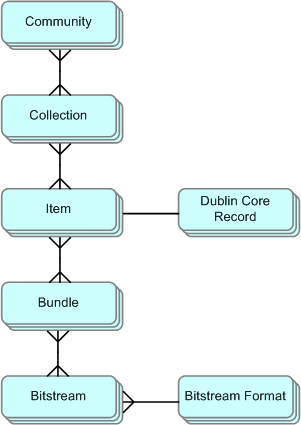
\includegraphics[scale=0.7]{images/data-model.png}
                            \end{center}
                            \caption{Daten-Modell}
                            \label{fig:dspace_data_model}
                        \end{figure*}\par
                \subsubsection{Authorisierung}
                    Es gibt zwei verschiedene Benutzergruppen :\\
                    \begin{enumerate}
                        \item{Administrator:}
                            Keine Einschr�nkungen.
                        \item{Anonymous:}
                            standardm��ig nur Lese-Zugriff.
                    \end{enumerate}
                    Es k�nnen Zugriffs-Policies f�r bestimmte Objekte angelegt werden. Somit ist es also m�glich �ber bestimmte Collections hinweg, Zugriffsbestimmungen zu schaffen.
                \subsubsection{Handles}
                    Ein \index{Handle}Handle ist ein wesentliches Feature von DSpace, welches es erm�glicht f�r Objekte eine eindeutige speicher- und ortsunabh�ngige ID zu vergeben, damit z.B. Zitate nicht ihr Zielobjekt verfehlen - im Falle einer Umsturkturierung der Webseite, auf der das zitierte Dokument liegt.
                \subsubsection{Such- und Browserdienste}
                    Das Auffinden von Ressourcen kann in drei verschiedenen Wegen angegangen werden :\\
                    \begin{enumerate}
                        \item{�ber eine externe Referenz(Handle)}
                        \item{�ber eine Stichwortsuche}
                        \item{Browsen �ber Title, Datum und Author}
                    \end{enumerate}
                \subsubsection{OAI-Support}
                    DSpace unterst�tzt das \index{OAI-PMH}OAI-PMH(Open Archives Protokoll for Metadata Harvesting), welches unter \url{http://www.openarchives.org/OAI/openarchivesprotocol.html}\cite{oai_pmh} zu einzusehen ist. Es dient der anwendungsunabh�ngigen Interoperabilit�t.
                \subsubsection{OpenURL-Support}
                    DSpace unterst�tzt das \index{OpenURL}OpenURL-Protokoll, welche Beschreibung unter \url{http://www.sfxit.com/OpenURL/} zu finden ist. Das OpenURL-Protokoll ist ein Protokoll f�r die Interoperabilit�t zwischen einer Informations-Ressource und einer Service-Komponente, die lokale Dienste in einer offenen Umgebung bereitstellt.\cite{openURL}
                \subsubsection{Quelle:} \url {http://dspace.org}            
            		\subsubsection{Fazit}
            			Dspace ist ein fortgeschrittenes Produkt, das viele gew�nschte Anforderungen schon beinhaltet. Weiterhin hat es sich im Einsatz bew�hrt(\url{https://dspace.mit.edu/index.jsp}). Anhand der Dokumentation jedoch schien die Umstellung der zu verwendenden Postgres-DB auf eine XML-Datenbank als Backend relativ kompliziert. Ausserdem w�rde sich eine recht hohe Einarbeitungszeit ergeben, die u.U. der Komplexit�t des anzugehenden Vorhabens nicht gerecht wird. Der entg�ltige Entschlu� fiel letztlich gegen Dspace als Basis-Produkt.
            \subsection{Greenstone}%Maxim
                Greenstone ist ein Software-Bundle, welches f�r die Erstellung und Verbreitung der Bibliothekscollections verwendet wird. Mit diesem Programm k{\"o}nnen
		Collections, die aus verschiedensten Dokumenten (B{\"u}cher, Artikel, Video, Audio) bestehen, erstellt und verwaltet werden. Eine gew{\"o}hnliche digitale Bibliothek, die mit Greenstone erstellt wurde, enth{\"a}lt mehrere Collections, die unterschiedlich organisiert sind, obwohl sie viel gemeinsam haben. Dar{\"u}ber hinaus k{\"o}nnen Collections leicht erg{\"a}nzt und umstrukturiert werden.
                \subsubsection{Suche nach Informationen}
                    Es existieren mehrere M{\"o}glichkeiten, wie die Suche nach Informationen gestaltet werden kann. Es kann nach einzelnen W{\"o}rtern, die entweder im gesamten
		    Text oder in bestimmten Teilen enthalten sind gesucht werden, sowie auch nach Titel oder einer bestimmten Thematik. Die {\"a}u{\ss}ere Seite jeder Collection enth{\"a}lt eine kurze {\"U}bersicht und die Information {\"u}ber die Struktur der Collection. Greenstone unterst{\"u}tzt die Volltextsuche, sowie auch die Indexsuche anhand der Metadaten. Diese Index werden w{\"a}hrend des Aufbauen der Collection erstellt.
                \subsubsection{Formate}
                    Greenstone unterst{\"u}tzt viele verschiedene Formate, die mit Hilfe der Plugins in ein standardisiertes Format {\"u}bersetzt werden: XML. Die Plugins die
		    Greenstone bereits enth{\"a}lt sind die zum {\"U}bersetzen von einfachem Text, HTML, DOC, PDF sowie Usenet und E-Mail. Dar{\"u}ber hinaus k{\"o}nnen auch neue Plugins erstellt werden.
                \subsubsection{Multimedia und Mehrsprachigkeit}
                    Die Collections k{\"o}nnen Text, Bilder, Video und Audio Dateien enthalten. Diese sind entweder durch Links oder Metadaten miteinander verbunden, was die M{\"o}glichkeit zur Volltextsuche erleichtert. Greenstone benutzt den Unicode, was f{\"u}r die richtige Verarbeitung und Darstellung der verschiedenen Sprachen erforderlich ist. Beim Arbeiten mit Collections, die in unterschiedlichen Sprachen verfasst sind, werden die einzelne Dokumente automatisch in der richtigen Sprache dargestellt.
                    \paragraph{Quelle:} \url{http://www.greenstone.org/cgi-bin/library}      

            \subsection{DLP - Distributed Library Project}%Jurij
            Distributed Library Project (kurz DLP) \index{DLP - Distributed Lybrary Project} ist eine Austauschplattform f{\"u}r B{\"u}cher, Videos und Tondokumente. \cite{DLP02}
              \subsubsection{Installation} 
          Im Normalfall ist eine Installation nicht notwendig. Im Internet existieren bereits mehrere DLP-Knoten, die so genannten Nodes, die nach dem Anlegen eines Benutzerkontos vollen Zugriff auf die wichtigsten Funktionen der Plattform erlauben. Alternativ l�sst sich die Plattform auch in Form eines komprimierten Archivs herunterladen, auf eigenem Host installieren und als weiteren Knoten betreiben. 
         \subsubsection{Benutzung und Funktionen} Unabh�ngig davon, ob man einen eigenen  Knoten einrichtet oder sich bei einem bereits bestehendem anmeldet, stehen den Benutzer folgende Funktionen zur Verf�gung \cite{DLP02}:
\begin{itemize}
	\item Medien katalogisieren\\
		Hierbei lassen sich  B�cher, Videos und Musik per Formular in eigene Listen aufnehmen und verwalten.
	\item Leselisten\\
		Mit dieser Funktion lassen sich B�cher verwandter Thematik zusammenfassen. 
	\item Status-Kontrolle\\
		Hier werden alle ausgeliehenen und entliehenen Medien auf einer Seite zusammengefasst.
	\item Suche nach neuen Medien\\
		Suchmaske nach Medien, die innerhalb des vorgegebenen Zeitraumes neu hinzugekommen sind. Zus�tzlich Auflistung aller neuen Mitglieder f�r denselben Zeitraum.
	\item Profil bearbeiten\\
		Hier lassen sich die bei der Anmeldung angelegte Profildaten jederzeit editieren.
	\item Benutzer suchen\\
		Es ist m�glich nach Benutzern mit gleichen Interessen, in der n�heren Umgebung oder nach einem zutreffenden Profil zu suchen.
	\item B�cher suchen\\
		Die B�cher lassen sich nach Autor, Titel und Besprechung suchen. Die genannten Attribute lassen sich auch einzeln anwenden. Dar�ber hinaus existiert ein Formular
		f�r die erweiterte Suche, wo weitere Attribute wie Gebiet, Eigent�mer und die Entfernung spezifiziert werden k�nnen. Die Browser- bzw. Suchergebnis-Ansicht listet
		die Ergebnisse mit Angabe des Besitzers, Autor und Titel des Buches, Verf�gbarkeitsstatus' sowie der geografischen Entfernung zum Buch.
	\item Empfohlene B�cher\\
		Diese Funktion versucht eine auf der eigenen B�chern basierte Liste der Interessen des Benutzers zu erstellen. Je mehr B�cher dieser verf�gbar macht, desto
		bessere Ergebnisse werden erzielt.
	\item Videos und Musik suchen\\
		Die Suche nach Audio und Video gestaltet sich �hnlich. Abh�ngig vom Medientyp stehen dann unterschiedliche Attributeingabefelder bereit.
\end{itemize}
 \subsubsection{Fazit}Die Oberfl�che ist unkompliziert und aufger�umt gehalten. Sie l{\"a}sst sich intuitiv bedienen, weil wirklich nur die grundlegendsten Funktionen
 implementiert wurden. Leider existiert kein Offline-Client. Um die B�cher verwalten zu k�nnen bzw.  nach Medien suchen zu k�nnen, muss sich der Benutzer online befinden. DLP
 implementiert keinen OAI-Protokoll. Die Suche nach DC-konformen Metadaten ist nicht m�glich. Die Daten eines Knoten werden in einer eigenen relationalen Datenbank in Form von
 Tabellen gehalten. Dabei sind die Datenbest�nde weitgehen unabh�ngig. Sowohl Anzahl der angemeldeten Benutzer als auch die Informationen �ber angemeldete Medien beziehen sich
 jeweils nur auf den Knoten auf welchem der Benutzer gerade aktiv ist. F�r jeden neuen Knoten ist eine weitere Registrierung notwendig. Somit wird es unm�glich, die
 Zusammenfassung aller knoten�bergreifenden Medien und Benutzer abzufragen.
                         \begin{figure*}[!hbt]
                            \begin{center}
                                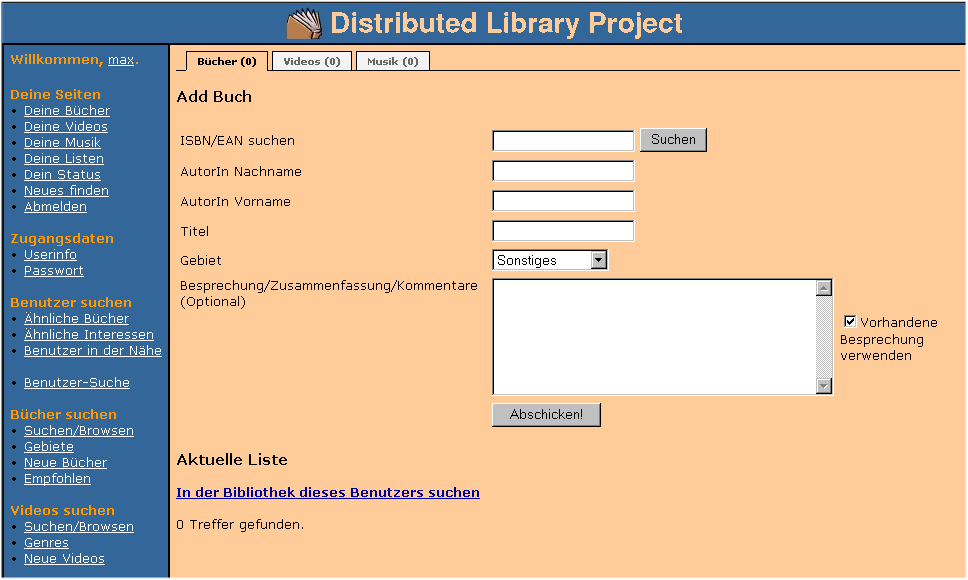
\includegraphics[scale=0.5]{images/dlp.png}
                            \end{center}
                            \caption{DLP-Oberfl�che}
                            \label{fig:dlp-desktop}
                        \end{figure*}\par
                        
                \subparagraph{Quelle:} \url {http://www.thoughtcrime.org/software/dlp/}

                \section{Programmiersprachenevaluation}
            In dem Projektvorhaben wird eine Standalone-Applikation erstellt. Um die Programmiersprache festzulegen wird ein projektunabh�ngiger Prototyp in vier verschiedenen Programmiersprachen erstellt. Der Prototyp ist eine GUI-Applikation mit folgenden Eigenschaften :
            \begin{itemize}
                \item{Men�leiste mit den Men�s 'Datei'}
                \begin{itemize}
                    \item{�ffnen (Dummy)}
                    \item{Speichern (Dummy)}
                    \item{Beenden}
                \end{itemize}
                \item{und dem Men� 'Hilfe'}
                \begin{itemize}
                    \item{Info (Popup-Fenster mit Informationen �ber Autor etc.)}
                \end{itemize}
            \end{itemize}
            Zur Erleichterung der Auswahl wird jede Applikation dokumentiert und anschlie�end eine
            Entscheidung �ber die Wahl der Programmiersprache getroffen.
            \subsection{Tcl/Tk}%Stefan
                \subsubsection{Allgemein}
                    \index{Tcl}Tcl steht f�r \textit{Tool Command Language}, wird 'tickle' ausgesprochen und ist eine Skriptsprache, die plattformunabh�ngig erstellt werden kann. Mittels des Interpreters wish (window shell) wird dann die erstellte Datei mit Endung '.tcl'
                    interpretiert und gestartet.\\
                    \index{Tk}Tk steht f�r \textit{Toolkit} und ist eine Erweiterung zu Tcl um grafische Elemente, wie die Erstellung einer GUI mit den jeweiligen Komponenten. Tk ist als Erweiterung zu verstehen, da es von verschiedenen Skriptsprachen benutzt werden kann (u.a. Perl/Tk).
                \subsubsection{Systemvoraussetzungen}
                    Tcl/Tk wird als Bundle kostenlos auf folgender Webseite angeboten : 
                    \url{http://dev.scriptics.com/software/tcltk/8.4.html}\\
		\subsubsection{Umsetzung}
		    Nach erfolgreicher Installation k�nnen direkt die mitgelieferten Demos als Argument des \textit{wish}-Interpreters aufgerufen werden. Somit fiel der
		    Einstieg recht leicht. Da in der Programmiersprache Tcl �berhaupt keine Kenntnisse vorlagen, wurde eine einfachen Textausgabe angefangen. Die ersten
		    Ergebnisse wurden sofort erzielt. Die speziellen Eigenschaften, wie das Action-Handling und die Modifikation von textuellen Elementen w�hrend der
		    Laufzeit erwiesen sich jedoch, auch auf Grund nicht bereit stehender Dokumentation, als gew�hnungsbed�rftig. Insgesamt hat das Erstellen des Demos ca.
		    5-8 Stunden gedauert, Feinheiten wie Shortcuts ausgeschlossen. Zur Betrachtung des Source-Codes sei auf den Anhang \ref{eval_tcl} verwiesen.
		\subsubsection{Screenshots}
                    Im Folgenden wird die anfangs beschriebene Funktionalit�t durch Screenshots belegt Bild(\ref{fig:easyButton_standard}),Bild(\ref{fig:easyButton_buttonpressed}),Bild(\ref{fig:easyButton_info}),Bild(\ref{fig:easyButton_hinweis}).
                    \begin{figure*}[!htb]
                        \begin{center}
                            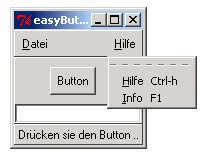
\includegraphics[scale=0.6]{images/easyButton_1.jpg}
                        \end{center}
                        \caption{EasyButton mit aufgeklappten Hilfe-Men�}
                        \label{fig:easyButton_standard}
                    \end{figure*}\par
                    \begin{figure*}[!htb]
                        \begin{center}
                            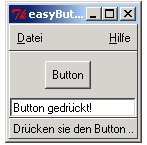
\includegraphics[scale=0.6]{images/easyButton_2.jpg}
                        \end{center}
                        \caption{EasyButton nach Bet�tigung des Buttons}
                        \label{fig:easyButton_buttonpressed}
                    \end{figure*}\par
                    \begin{figure*}[!htb]
                        \begin{center}
                            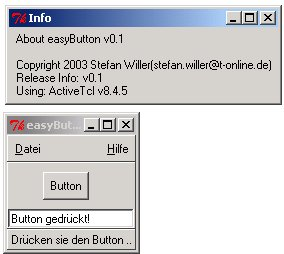
\includegraphics[scale=0.6]{images/easyButton_3.jpg}
                        \end{center}
                        \caption{EasyButton mit Info-Dialog}
                        \label{fig:easyButton_info}
                    \end{figure*}\par
                    \begin{figure*}[!hb]
                        \begin{center}
                            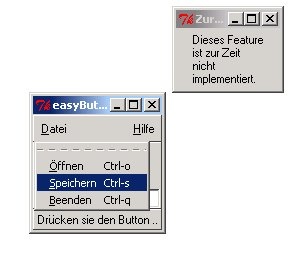
\includegraphics[scale=0.6]{images/easyButton_4.jpg}
                        \end{center}
                        \caption{EasyButton mit Hinweis}
                        \label{fig:easyButton_hinweis}
                    \end{figure*}\par
								\subsubsection{Fazit}
									Tcl/Tk ist �u�erst geeignet, um schnell einfache Gui's(\textit{g}rafical \textit{u}ser \textit{i}nterface) zu erzeugen. Die Anbindung an andere Datenquellen und der unterschiedliche Einsatz (z.B. standalone vs. embedded) wurde hierbei nicht untersucht. Es kann abschliessend also kein Pro oder Contra ausgesprochen werden.
						\newpage
            \subsection{Java}%Frank
                \subsubsection{Allgemein}
                    Java ist eine plattformunabh�ngige Programmiersprache der Firma Sun Microsystems. Als
					Standardwerk zum Thema Java hat sich \cite{goto_java2} einen Namen gemacht.
                \subsubsection{Voraussetzungen}
                    Um die Programme ausf�hren zu k�nnen, ist die Installation einer Java Laufzeitumgebung (JRE) notwendig. F�r das eigene Erstellen von Programmen wird eine Compilerumgebung ben�tigt (SDK). Java ist auf sehr vielen Computern bereits installiert und damit weit verbreitet. Die aktuelle Version beider Umgebungen kann kostenlos unter \url{http://java.sun.com/j2se/1.4.2/download.html} heruntergeladen werden.
                \subsubsection{Implementation}
                    Das Testprogramm wurde mit Hilfe der Swing-Bibliotheken erstellt. Das Men� enth�lt die Eintr�ge: �ffnen, Speichern und Beenden. Tooltips erleichtern die Bedienung. Ein Tooltip gibt eine kurze Hilfe aus, wenn der Mauszeiger �ber einem Objekt (z.B. Knopf) stehen bleibt. F�r die Implementation wurde das JDK von Sun in der Version 1.4.2 verwendet. Als Entwicklungsumgebung wurde das freie Softwarepaket
					Eclipse \url{http://www.eclipse.org}
					von der Firma IBM eingesetzt. Das kompilierte Programm wurde erfolgreich unter Windows, Linux und FreeBSD getestet.
				\subsubsection{Bewertung}
				Die Programmierung gelang z�gig aufgrund der Einfachheit von Java und der ausgereiften
				Entwicklungsumgebung Eclipse. Durch die Plattformunabh�ngigkeit von Java war das Testprogramm
				ohne Anpassungen auf verschiedenen Betriebssystemen sofort lauff�hig. Java ist daher ein 						geeigneter Kandidat f�r die	Implementierung.
                \subsubsection{Screenshots}
                    \begin{figure*}[!htb]
                        \begin{center}
                            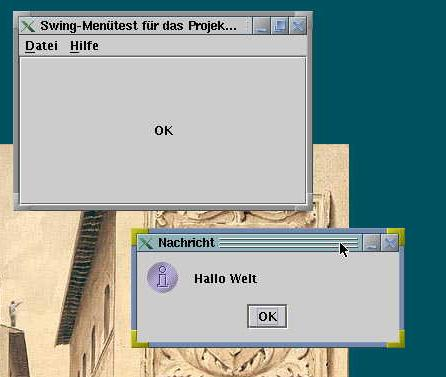
\includegraphics[scale=0.5]{images/java-guitest-screenshot-linux.jpg}
                        \end{center}
                        \caption{Die HalloWelt-Oberfl\"ache mit  Java unter Linux}
                        \label{fig:hallo_standard_1}
                    \end{figure*}\par

            \subsection{C\# mit Mono und GTK\#}%Thorsten
                \subsubsection{Allgemein}
                    C\# wurde von Microsoft entwickelt und ist eine halb compilierte, halb interpretierte Programmiersprache \"ahnlich wie Java. Als Entwicklungsvoraussetzung wird das .Net-Framework von Microsoft ben�tigt. Es gibt allerdings mit einem Projekt namens "`\textit{Mono}"' eine Open-Source Implementation des .Net-Frameworks. \textit{Mono} wurde f\"ur diesen C\# Test verwendet.
                \subsubsection{Systemvoraussetzungen}
                    \textit{Mono} enth\"alt alle Developmenttools, die f\"ur die C\# Programmierung ben�tigt werden, insbesondere den Compiler und die Laufzeitumgebung. Des weiteren wird in diesem Test GTK\# zur Erstellung der grafischen Oberfl\"ache verwendet.\\
                    \noindent \url{http://www.go-mono.com/} \\
                    \url{http://gtk-sharp.sourceforge.net/}
                \paragraph{Umsetzung}
                    \begin{itemize}
                        \item{Windows} \\
                            F\"ur Windows existiert ein Installationsprogramm mit dem sich \textit{Mono} problemlos installieren lie\ss. C\# verwendet standardm\"a{\ss}ig das
			    "`Windows.Forms"' Toolkit, das aber Windows-nativ ist und da dieser Test auch auf Linux-Systemen laufen soll, wurde das GTK\# verwendet, welches f\"ur
			    beide Plattformen erh\"altlich ist. GTK\# lie\ss sich ebenfalls reibungslos installieren, allerdings ist die Dokumentation (noch) nicht vollst\"andig, was zu m\"uhseligem Ausprobieren ("`Trial \& Error"') der bereitgestellten Methoden f\"uhrte.
                        \item{Linux(Debian)}\\
                            Da f\"ur \textit{Mono} ein Debian-Paket vorhanden war, verlief die Installation ebenfalls unkompliziert. GTK\# ben\"otigt allerding GTK 2.0 (auf dem Testsystem war nur 1.3 vorhanden), und dieses verlangte wiederum weitere Pakete, was eine langwierige Installation mit leichten Hindernissen zur Folge hatte. Der bereits unter Windows erstellte Quellcode lies sich dann aber problemlos compilieren und ausf\"uhren.
                    \end{itemize}

                    \begin{figure*}[!htb]
                        \begin{center}
                            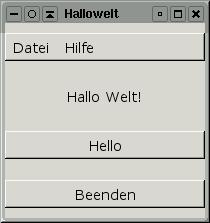
\includegraphics[scale=0.6]{images/c-sharp_gtk_linux_pic1.jpg}
                        \end{center}
                        \caption{Die HalloWelt-Oberfl\"ache mit C\# unter Linux}
                        \label{fig:hallo_standard_2}
                    \end{figure*}\par

                    \begin{figure*}[!htb]
                        \begin{center}
                            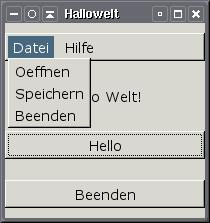
\includegraphics[scale=0.6]{images/c-sharp_gtk_linux_pic2.jpg}
                        \end{center}
                        \caption{Die HalloWelt-Oberfl\"ache mit aufgeklappten Datei-Men\"u}
                        \label{fig:hallo_menu}
                    \end{figure*}\par   

            \subsection{PHP-Gtk}%Jurij,Maxim
            \subsubsection*{Allgemein}
             PHP (Akronym f�r "`PHP: Hypertext Preprocessor"')\index{PHP} ist eine weit verbreitete und f�r den allgemeinen Gebrauch bestimmte Open Source Skriptsprache, welche speziell f�r die Webprogrammierung geeignet ist, und in HTML eingebettet werden kann. PHP-GTK ist eine PHP-Erweiterung zur Programmierung und Erstellung von GUI-Oberfl�chen (Graphical User Interface) mit der GTK+-Bibliothek bereit.\cite{PHP01}
             \subsubsection*{Systemvoraussetzungen}
             PHP gibt es sowohl f�r Unix als auch f�r die Windows{95/98/NT}-Plattformen, sehr verbreitet ist die Integration von PHP als Modul in den Apache-Webserver
	     (\url{http://www.apache.org}), des weiteren ist die Ausf�hrung �ber CGI m�glich. Die Adressen des PHP-Projektes: \url{http://www.php.net}, \url{http://www.php3.de}
	     oder auch \url{http://de.php.net}. Dort befindet sich PHP selbst (als vorkompilierte Version oder Quelltext), die englischsprachige Dokumentation sowie weitere
	     Informationen zu englischsprachigen Mailinglisten, etc..
	     
	       \subsubsection{Umsetzung}%Jurij
	      Die \index{phpGTK} phpGTK-Bibliothek stellt eine Reihe an objekt-orientierten Schnittstellen zu den GTK+ Klassen und Funktion und soll so die Entwicklung von clientseitigen GUI-Anwendungen. \cite{PHPGTK01}
	    Die GTK+-Bibliothek wurde noch k�rzlich in der der neuen 1.0.0er Version(davor v0.5.1) zum Download freigegeben. Sie soll in erster Linie m�glichst gr��te Kompatibilit�t zu PHP4 gew�hrleisten und ein F�lle an Bugs der Vorversion beseitigen.\\

	   Das Download-Archiv ist etwas �ber drei Megabyte gro� und enth�lt die Funktionsbibliotheken sowohl f�r die Windows als auch f�r die Linux/Unix Plattformen. Installation ist nicht notwendig, das Archiv l�sst sich problemlos entpacken. Lediglich  die Konfigurationsdatei der PHP-Umgebung muss angepasst werden. Entsprechende vorkonfigurierte Dateien werden aber mitgeliefert. \\
	   
	   Im Paket sind  zahlreiche, zum Teil ausreichend kommentierte, Skriptbespiele vorhanden, die sich unproblematisch Ausf�hren lassen. Mit deren Hilfe lassen sich die meisten wichtige Funktionen schnell erlernen. Die Programmierung erfolgt stets mit der PHP-Syntax, was die Arbeit f�r erfahrene PHP-Programmierer sicherlich erleitert. Der cose-seitige Prinzip des GUI-Layouts ist leicht mit dem von den bekannten Java-Layoutmanagern verwandt, erreicht allerdings bei weitem nicht deren Flexibilit�t. Daher sind die erreichbaren Ergebnisse optisch nicht sehr ansprechend.\\
	   
	   Der mitgelieferte ausf�hrbare \index{phpGTK-Interpreter} Interpreter nimmt  GTK-konforme PHP-Skipte  als Argumente per eine Shell-Komandozeile auf, hat jedoch einen sehr gravierenden Mangel. Es gibt keinen aus dem Web-PHP bekannten Pre-Parser. Bei den geringsten Fehlern, wie zum Beispiel dem fehlenden Semikolon, wird die Skriptabarbeitung ohne einzige (Fehler-)Meldung abgebrochen. Bei einem anspruchsvollen und umfangreichen Projekt w�re dies ein festes KO-Kriterium. Das Gleiche passiert auch, wenn ein Laufzeitfehler auftritt. Die Anwendung an sich ist nicht besonders performant und kann sogar als leicht tr�ge bezeichnet werden. Die Performanz der PHP-GTK-Anwendungen kann zweifelsfall mit den von Javaanwendungen verglichen werden, ohne dass die aus Java bekannte Funktionsvielfallt zur Verf�gung steht.\\
	   
	   Die Dokumentation ist zwar vorhanden und zum Teil auch hilfreich, allerdings ist sie nach wie vor auch in der englischen Originalfassung unvollst�ndig. Die deutsch-sparachige Dokumentation ist unbrauchbar, da sie nur zu einem geringen Prozentsatz �bersetz wurde. Die restlichen Passagen wurden der Originalfassung entnommen.
	\newpage
	     \subsubsection{Screenshots}
						
                    \begin{figure*}[!htb]
                        \begin{center}
                            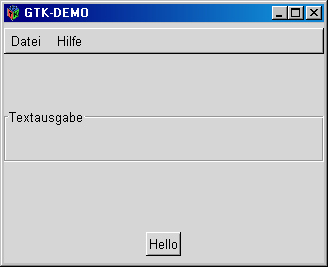
\includegraphics[scale=0.6]{images/shot1.jpg}
                        \end{center}
                        \caption{Die HalloWelt-Oberfl\"ache mit PHP-GTK}
                        \label{fig:hallo_standard_3}
                    \end{figure*}\par
                    

                    \begin{figure*}[!htb]
                        \begin{center}
                            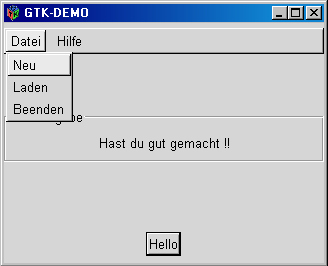
\includegraphics[scale=0.6]{images/shot3.jpg}
                        \end{center}
                        \caption{Die HalloWelt-Oberfl\"ache mit aufgeklappten Datei-Men\"u}
                        \label{fig:hallo_standard_4}
                    \end{figure*}\par
                    

                    \begin{figure*}[!htb]
                        \begin{center}
                            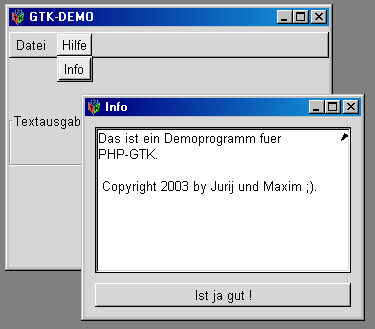
\includegraphics[scale=0.6]{images/shot2.jpg}
                        \end{center}
                        \caption{Die HalloWelt-Oberfl\"ache mit aufgeklappten Info-Men�}
                        \label{fig:hallo_standard_5}
                    \end{figure*}\par

        \section{Signaturbildung}%Thorsten  
\index{Signaturbildung}
\subsection{Signaturbildung im Bibliothekswesen}

Im Bibliothekswesen bezeichnet die Signatur \index{Signatur} den Standort eines Buches \index{Buch} in der \index{Bibliothek} 
Bibliothek \cite{signatur_begriff}.
Eine solche Signatur ist eineindeutig: es gibt f\"ur \textit{jedes} Exemplar eines Buches eine
eindeutige Signatur, selbst wenn von dem Buch mehrere identische Kopien existieren.

Zur Bildung einer solchen Signatur gibt es verschiedene Ans\"atze; an dieser Stelle
sollen zwei grob beschrieben werden: die Signaturbildung anhand der \textit{Bremer Systematik} \index{Bremer Systematik}und der 
\textit{Regensburger Verbundklassifikation}. \index{Regensburger Verbundklassifikation}

\subsubsection{Bremer Systematik}

Die Bremer Systematik oder auch Bremer Fachsystematik kommt zum einen (nat\"urlich) an
der Staats- und Universit\"atsbibliothek Bremen, aber auch an der hiesigen Bibliothek der
Carl von Ossietzky Universit\"at Oldenburg zum Einsatz. Anhand der Fachsystematik wird
die Signatur gebildet, indem ein K\"urzel des Fachs als zentrales Element in die Signatur
\"ubernommen wird. Die Bremer Fachsystematik ist online zu finden unter \cite{fachsystematik}.
An der Bibliothek der Universit\"at Oldenburg wird die Signatur mit Hilfe der Systematik wie
folgt gebildet:

\begin{itemize}

\item drei Buchstaben, die das Fach angeben (``Fachzuweisung''),
\item einer Zahlenkombination, die die Systemstelle (bzw. das Fachgebiet)
    innerhalb des Faches angibt (``systematische Notation'') und
\item einer ``Aufstellungsnummer'', bestehend aus zwei Buchstaben und vier Ziffern.

\end{itemize}

\noindent \textbf{Beispiel:} Bsp: inf 724 CK 5213 



\subsubsection{Regensburger Verbundklassifikation}

Als Studenten der Carl von Ossietzky Universit\"at war es f\"ur uns naheliegend, die Bremer Systematik
zu verwenden. Dennoch wurde im Vorfeld auch die Signaturbildung anhand der Regensburger Verbundklassifikation 
betrachtet, die der Vollst\"andigkeit halber hier kurz beschrieben wird. 
Eine Online-Version der Klassifikation findet sich unter \cite{rvk}.
Die Signatur besteht aus \cite{sig_regensburg}:
\begin{itemize}
\item einem Lokalkennzeichen (2-3 Ziffern), gefolgt von einem Schr\"agstrich ('/'),
\item einer Systemstelle (2 Grobuchstaben + mehrstellige Zahl), die sich anhand der Klassifikation ergibt
\item und einem individualisierenden Element (Cluster-Sanborn-Notation bzw. 
   Erscheinungsjahr, ggf. noch Auflage, Band, Exemplar).
\end{itemize}

\noindent \textbf{Beispiel:} 17/GE 4001 B724 (9) -2 +3

\subsection{Signaturbildung im Projekt}

\subsubsection{Allgemeines}

Als Signatur zur Kennzeichnung der verschiedenen Exemplare des
Bibliotheksbestand orientieren wir uns an der sogenannten "'Bremer Systematik"',
indem wir die von ihr verwendeten Fachk\"urzel (bzw. Fachzuweisungen) 
als Voreinstellung f\"ur die Kategorien \index{Kategorie}anbieten.
Die von uns verwendete Signatur setzt sich wie folgt zusammen:

\begin{itemize}

    \item drei Buchstaben, die das Fach angeben ("'Fachzuweisung"'),

    \item gefolgt von einem Unterstrich ("'\_"'),
    
    \item und einer laufenden Nummer von 1 bis 999999999, die hexadezimal dargestellt wird, also
      bis 2540BE3FF. Durch die hexadezimale Darstellung soll die Lesbarkeit der Nummer 
      erh\"oht werden.
    
\end{itemize}




\subsubsection{Algorithmus zur Signaturbildung} \index{Signaturbildung}
    
    \begin{enumerate}
        
        
          
        \item Bestimme das Fachgebiet \index{Fachgebiet} anhand der Bremer Systematik (oder sonstiger zur
          Verf\"ugung stehenden Kategorien) in Form eines
          K\"urzels aus drei Kleinbuchstaben

        \item H\"ange einen Unterstrich an das K\"urzel an
        
        
        \item Bestimme die fortlaufende Nummer des Gesamtbestandes wie folgt:
          \begin{itemize}
            
          \item Die erste Nummer des Bestands ist 000000001.
          
          \item Die letzte verwendete Nummer (die dem System bekannt sein muss) wird um
              eins erh\"oht und an die bisherige Signatur angef\"ugt.
          
          \end{itemize}

   \end{enumerate}
\textit {Hinweis:} Konsequenz des obigen Algorithmus ist, dass jedes Objekt der Datenbank 
eine eigene Signatur erh\"alt, also z.B. B\"ucher, die mit mehreren Exemplaren im Bestand
vorhanden sind, besitzen jeweils eine individuelle Signatur.

\subsection{URI, URN}

\subsubsection{Was sind URIs, URLs und URNs?}

URI \index{URI} ist die Abk\"urzung f\"ur \textit{Uniform Resource Identifier}. Ein URI ist eine kompakte
Zeichenkette zur Identifizierung einer abstrakten oder physikalischen Ressource \cite{rfc2396}.
Eine Ressource \index{Ressource} kann alles sein, was einen Namen hat oder beschrieben werden kann, z.B. Dokumente, 
Bilder oder ein Service.
Weiterhin versteht man unter URI den Oberbegriff f\"ur die Unterarten \textit{Uniform Resource Locator}(URL)
und \textit{Uniform Resource Name}(URN). 

URLs \index{URI} identifizieren eine Ressource \"uber den Ort (im WWW), an dem sie zu
finden ist, nicht \"uber einen Namen oder Attribute \cite{rfc2396}. Sie stellen also 
gewisserma{\ss}en einen Zeiger auf die Ressource dar.

URNs \index{URN} sollen als best\"andige, ortsunabh\"angige Bezeichner f\"ur Ressourcen dienen \cite{rfc2141}. Eine URN
bezeichnet eine Ressource eindeutig, d.h. ist sie mehrfach im Netz vertreten, besitzt sie immer
denselben URN, wo hingegen sie mehrere unterschiedliche URLs hat.

\subsubsection{Syntax}

\paragraph{Uniform Resource Identifier}

Die komplette Syntax von URIs ist im \index{Request for Comment} 'Request for Comment' (RFC) 2396 \cite{rfc2396} angegeben. 
An dieser Stelle wird
nur ansatzweise auf einige wichtige Merkmale eingegangen.

\begin{itemize}

\item Grunds\"atzlich sind nur Zeichen des US-ASCII Zeichensatzes erlaubt. Davon abweichende Zeichen k\"onnen
  mit Hilfe des ``Escape''-Zeichens '\%' benutzt werden.

\item Jeder URI beginnt mit dem Namen eines Schemas, bestehend aus einer Zeichenfolge, die mit ':' abschliesst, 
z.B. ``http:'' oder ``ftp:''.

\item Ein URI ist wie folgt aufgebaut (Auszug):

  \begin{verbatim}
    URI       = scheme ":" hier_part [ "?" query] 
                ["#" fragment]
    
    hier_part = net_path | abs_path | rel_path
    
    net_path  = "//" authority [ abs_path ]
    abs_path  = "/" path_segments
    rel_path  = rel_segments [ abs_path ]

    ...

  \end{verbatim}

\end{itemize}

\noindent \textbf{Beispiel:} $\underbrace{foo}_{scheme}:\underbrace{//example.com:8042}_{authority}
\underbrace{/over/there}_{path}?\underbrace{name=ferret}_{query}\#\underbrace{nose}_{fragment}$


\paragraph{Uniform Resource Name}

Alle URNs haben die gleiche Syntax \cite{rfc2141}:

\begin{verbatim}

  <URN> ::= "urn:" <NID> ":" <NSS>

\end{verbatim}

NID bedeutet \textit{Namespace Identifier}. Ein Namespace (Namensraum) ist eine Menge von einheitlichen
Bezeichnern. Ein NID beginnt mit einem Buchstaben oder einer Zahl gefolgt von einer Folge aus 
Buchstaben, Zahlen und dem '-' Zeichen. Gro{\ss} und Kleinschreibung wird nicht unterschieden.

NSS bedeutet \textit{Namespace Specific String}. Er besteht aus Buchstaben, Zahlen, reservierten
Zeichen ('\%', '/', '?', '\#') und weiteren Sonderzeichen\footnote{f\"ur Details siehe \cite{rfc2141}}.
Bei den reservierten Zeichen ist zur Zeit nur '\%' gebr\"auchlich, die anderen wurden reserviert f\"ur
eine zuk\"unftige Nutzung, sollen aber im Moment nicht benutzt werden.

\noindent \textbf{Beispiel:} $\underbrace{urn}_{scheme}:\underbrace{example:animal:ferret:nose}_{path}$


\subsection{Kategorisierung von Dokumenten}

Eine Kategorie \index{Kategorie} besteht in \textit{Tooliban} aus einem (die Kategorie beschreibenden) Wort und einer
aus diesem Wort abgeleiteten Abk\"urzung, die aus drei Kleinbuchstaben besteht und in die Signatur \index{Signatur}
von Objekten \index{Objekt} aufgenommen wird, die dieser Kategorie zugeordnet werden. \textit{Tooliban} enth\"alt 
eine vorgefertigte Liste von Kategorien. Diese Kategorien entsprechen den F\"achern und Fachk\"urzeln 
der \index{Bremer Systematik} 'Bremer Systematik'. Zus\"atzlich gibt es noch eine Kategorie 'not available' f\"ur alle
Objekte, die keiner Kategorie zugeordnet werden k\"onnen.

Des Weitern ist es Personen mit administrativem Zugang zur Datenbank gestattet, weitere Kategorien 
hinzuzuf\"ugen. Das Entfernen von Kategorien ist allerdings nur erlaubt, wenn noch kein Objekt (z.B. Buch)
innerhalb dieser Kategorie erstellt wurde. Der Grund daf\"ur ist, dass nach der Erstellung eines 
Eintrages eine Signatur gebildet wird, die das Kategorienk\"urzel beinhaltet. Um die Eineindeutigkeit
der Signatur zu gew\"ahrleisten, ist ein Entfernen der Kategorie nicht mehr m\"oglich.


                 \section{XML als Beschreibungssprache}%Frank
		\subsection{Was ist XML?}
		XML steht f�r 'Extensible Markup Language' und ist eine beschreibende
		Sprache. Sie stellt einen Standard dar, mit dem Dokumente beschrieben und
		verarbeitet werden k�nnen. Die Sprache XML wurde wie HTML vom World Wide Web
		Consortium \cite{xml_w3c} geschaffen und ist eine vereinfachte Variante der
		Standard Generalized Markup Language (SGML). Nach \cite{xml_practical} ist XML
		die neue Sprache f�r das Web.
		Als Meta-Sprache ist es ohne
		statische Vorgaben m�glich, Tags selbst zu definieren, z.B.: $<$Buchbesprechung$>$
		oder $<$Geburtstag$>$. Die Elemente k�nnen durch Document Type Definitions (DTD)
		deklariert und beschrieben werden.
		\subsection{Warum XML f�r das Projekt 30?}
		Die Spezifikation von XML ist frei verf�gbar, ohne die Rechte Dritter zu verletzen. Damit erf�llt es
		die Anforderungen f�r das Modul 'Virtuelle Organisation - Open Source' und ist vollst�ndig
		dokumentiert. Weiterhin erm�glicht XML die strukturierte Darstellung von Daten und beseitigt damit einige der Schw�chen von HTML. Die Anforderungen der Auftraggeber lassen eine objektorientierte 		Datenhaltung sinnvoller erscheinen. Eine XML Datenbank kann daher die anfallenden Daten besser 			aufnehmen als eine relationale Datenbank. XML Dateien lassen sich leicht validieren und auch �ber 		langsame Netzwerkverbindungen performant �bertragen. Ganze B�cher dokumentieren den Einsatz von XML und Datenbanken, z.B. \cite{xml_database}.
			\subsubsection{Terminologie}
			Ein XML Dokument besteht aus mindestens einem Element, das z.B. folgende Form
			hat:
			\begin{center}
			  \begin{verbatim}
			    <Kopfzeile>
			       Hier steht die Kopfzeile.
			    </Kopfzeile>
			  \end{verbatim}
			\end{center}
			Das Element Kopfzeile hat ein �ffnendes und eine schlie�endes Tag. Ein
			Element beginnt mit dem Symbol f�r die �ffnende spitze Klammer ($<$) und endet mit dem
			Symbol f�r die schlie�ende spitze Klammer ($>$). Das schlie�ende Tag ist bis auf ein Symbol
			identisch: vor dem Namen des Elementes befindet ein Slash (/), mit diesem Tag
			endet die Beschreibung f�r ein Element. Weiterhing k�nnen auch Attribute definiert werden:
			\begin{center}
			  \begin{verbatim}
  			    <L�nge L�ngenma�="cm">16,8</L�nge>
			  \end{verbatim}
			\end{center}
			Das Attribut wird hier innerhalb des �ffnenden Tags definiert und hei�t
			L�ngenma�. Dem Attribut wird die Eigenschaft 'cm' zugewiesen. Die Eigenschaft
			steht innerhalb von Anf�hrungsstrichen. Es gibt weiterhin auch Tags ohne
			Inhalt, die nur ein Attribut definieren:
			\begin{center}
			  \begin{verbatim}
				<Quelle link="http://www.google.de"></Quelle>
				<Quelle link="http://www.google.de"/>
			  \end{verbatim}
			\end{center}
			Beide Elemente im Beispiel sind identisch, leere Elemente dienen h�ufig dazu,
			zus�tzliche Informationen zu �bertragen, die nicht direkt im Text
			stehen (sollen).

				\paragraph{Zwingende Eigenschaften von XML}
				Attribute m�ssen in Anf�hrungsstrichen stehen, auf das obige Beispiel
				bezogen w�rde:
				\begin{center}
				  \begin{verbatim}
				  <Quelle link=http://www.google.de/>
				    \end{verbatim}
				\end{center}
			zu einer Fehlermeldung f�hren.\\
			Jedes Element, das nicht leer ist, muss ein �ffnendes und ein schlie�endes
			Tag besitzen. Folgender Aufbau ist nicht erlaubt:
			\begin{center}
			  \begin{verbatim}
				<Tagespunkt>
				  1. Tagespunkt
				<Tagespunkt>
				  2. Tagespunkt
			  \end{verbatim}
			\end{center}
			Eine richtige Darstellung sieht folgenderma�en aus:
			\begin{center}
			  \begin{verbatim}
				<Tagespunkt>
				  1. Tagespunkt
				</Tagespunkt>
				<Tagespunkt>
				  2. Tagespunkt
				</Tagespunkt>
			   \end{verbatim}
				Elemente mit gleichem Namen d�rfen beliebig oft verwendet werden.
			\end{center}
			Tags m�ssen korrekt geschachtelt werden. Ein schlie�endes Tag muss auf
			das identische �ffnende Tag folgen, es mu� ihm am n�chsten stehen.
			Der folgende Aufbau stellt eine korrekte Schachtelung dar:
			\begin{center}
			  \begin{verbatim}
				<Tagespunkt>
				  <fettgedruckt>
				    1. Tagespunkt
				  </fettgedruckt>
				</Tagespunkt>
			  \end{verbatim}
			\end{center}
			w�hrend folgendes Beispiel eine Fehlermeldung erzeugt:
			\begin{center}
			  \begin{verbatim}
				<Tagespunkt>
				  <fettgedruckt>
				    1. Tagespunkt
				  </Tagespunkt>
				</fettgedruckt>
			  \end{verbatim}
			\end{center}
			\subsubsection{Namensr�ume}
			Namensr�ume l�sen Probleme, die bei gleichen Elementnamen auftauchen, die nicht zusammengeh�ren. Namensr�ume sind mit lokalen und globalen Variablen in der objektorientierten
			Programmierung vergleichbar. Beispiel:
			\begin{center}
			  \begin{verbatim}
				<birne>
				  <fassung>Blech</fassung>
				  <draht>Wolfram</draht>
				</birne>

				<obst>
				  <birne>Helene</birne>
				  <apfel>Braeburn</apfel>
				</obst>
			  \end{verbatim}
			\end{center}
			Wird ein Dokument erstellt, das beide Elemente zusammenf�hrt, so w�re unklar, welche Inhalte
			das Element '$<$birne$>$' haben darf. Das Problem wird dadurch gel�st, das den Elementen der
			Namensraum vorangestellt wird, getrennt durch einen Doppelpunkt.
			\begin{center}
			  \begin{verbatim}
			    <licht xmlns="http://www.lagerraum.de/">
			      <birne>Lichtquelle</birne>
			        <nahrung xmlns:obstkiste="http://www.lecker.de/">
			          <obstkiste:birne>Helene</obstkiste:birne>
			          <bewohner="M�use"/>
			        </nahrung>
			    </licht>
          		  \end{verbatim}
			\end{center}
			Die erste Definition $<$birne$>$ geh�rt zum Namensraum 'licht', da dieser zuletzt definiert wurde.
			Da kein Doppelpunkt in der Deklaration vorkommt, wird 'licht:' als Standardnamensraum
			angesehen. Um einen zweiten Namensraum schaffen zu k�nnen, wird dem Element 'nahrung' das Pr�fix 'obstkiste:' vorangestellt. So kann die zweite Definition von 'birne' eindeutig dem
			Namensraum 'obstkiste' zugewiesen werden. Wird kein Namensraum verwendet, so gilt wieder der
			Standardnamensraum, in diesem Fall 'licht'.


		\subsection{Dublin Core}
		Im Internet ist es nicht immer leicht, eine gew�nschte Information zu�
		finden. Es ist zuviel Information verf�gbar, das relevante Wissen muss�
		herausgefiltert werden. Zudem sind gleichartige Informationen, wie z.B.�
		eine Buchbeschreibung, nicht in gleichartigen Formaten gespeichert. Weiterhin fehlte �berhaupt
		ein Standard, der Daten �ber Daten enth�lt, also Dateien, die ein Bild oder ein Dokument
		beschreiben. Auf einer Konferenz sollte eine Einigung gefunden werden, um mit Hilfe von
		Metadaten einen Standard zu finden, mit dem Dokumente beschrieben werden k�nnen.
			\subsubsection{Entstehung des Dublin Core}
			In Dublin (Ohio) fand 1995 die erste Konferenz statt, auf der sich ein 'Metadata
			Workshop' mit der Definition von Elementen besch�ftigte, die einen Standard
			f�r die Dokumentenbeschreibung darstellen sollte. Der Name Dublin Core leitet sich
			vom ersten Tagungsort ab, inzwischen befindet sich die 'Dublin Core Metadata Initiative'
			unter \cite{dublin_core} im Internet. Das Ergebnis der ersten Tagung waren 13 Elemente,
			auf die sich die 50 Teilnehmer einigten. Auf der dritten Konferenz wurde festgelegt, das
			die Metadaten nicht nur auf Textdokumente, sondern auch auf Bilder und andere visuelle
			Objekte angewendet werden k�nnen. Der vierte Workshop ergab, das zu den inzwischen 15
			Elementen keine mehr hinzugef�gt werden sollen. Bei der Entwicklung stellte sich
			heraus, das Metadaten in der Sprache vorliegen, in der auch das zu beschreibende
			Dokument verfasst ist. Aus diesem Grund wurde Dublin Core und seine Elemente in �ber
			20 Sprachen �bersetzt, um den Interessenten aus �ber 50 L�ndern entgegen zu kommen.
			Die Standardsprache ist jedoch Englisch, gleiche Metatags d�rfen beliebig oft vorkommen.
			\subsubsection{Elemente des Dublin Core}
			Die 15 Metadatenelemente sind recht einfach gehalten, um gr��tm�gliche Flexibilit�t zu
			erreichen. Die Elemente enthalten Informationen �ber ein Dokument, um es zu kategorisieren
			und zu beschreiben. Dadurch wird eine Indizierung erst m�glich und die Suche in gro�en
			Datenbest�nden stark vereinfacht. Die Erfahrung zeigt, das alle Elemente sowohl auf B�cher,
			als auch auf Tondokumente oder Filme angewandt werden k�nnen. Die Elemente werden als
			'Dublin Core Metadata Element Set' bezeichnet, sie beginnen alle mit dem Pr�fix 'DC.'.
				\paragraph{1. DC.title}
				DC.title bezeichnet den Namen f�r das Dokument, also ein Buchtitel oder der Name von
				einem Film.
				\paragraph{2. DC.creator}
				Hiermit wird der Verfasser oder Urheber definiert, der f�r das Dokument intellektuell
				verantwortlich zeichnet. Dies kann ein Autor, aber auch ein Maler, Fotograf oder
				Komponist sein.
				\paragraph{3. DC.subject}
				Das dritte Element steht f�r das Thema, mit dem sich das Dokument auseinandersetzt.
				Hiermit sind auch Schlag- oder Stichworte gemeint, die den Inhalt beschreiben.
				Auch Phrasen oder das Thema des Dokumentes k�nnen hier erfasst werden.
				\paragraph{4. DC.descripton}
				Hier erfolgt eine inhaltliche Beschreibung in Textform. Dokumente im Textformat
				werden mit einer Inhaltsangabe beschrieben, graphische Objekte mit einer Art
				Inhaltsangabe.
				\paragraph{5. DC.publisher}
				Dieses Metatag definiert den Verleger oder Herausgeber, je nachdem, wer daf�r
				verantwortlich ist, dass das Dokument �berhaupt zur Verf�gung steht.
				\paragraph{6. DC.contributors}
				Beteiligte Personen und K�rperschaften werden hier aufgef�hrt. Allgemein die Personen,
				die irgendwie an dem Dokument mitgearbeitet haben, aber nicht direkt Autor sind.
				Dies sind z.B. �bersetzer oder Illustratoren.
				\paragraph{7. DC.date}
				In diesem Tag wird das Datum erfasst, an dem das Dokument verf�gbar gemacht wurde.
				Empfohlen wird eine 8-stellige Zahl im Format JJJJMMTT, wie es in ANSI X3.30-1985
				definiert ist. Beispielsweise steht 19720219 f�r den 19. Februar 1972.
				\paragraph{8. DC.type}
				Hier wird die Art beschrieben, in der das Dokument vorliegt etwa ein Buch, ein
				Musikst�ck oder ein Zeitungsartikel.
				\paragraph{9. DC.format}
				Das Dokumentformat wird im neunten Metatag erfasst. Hierbei wird das technische
				Format angegeben, in der das Dokument vorliegt. Das kann z.B. die Papierform sein,
				wenn es sich um ein Buch handelt oder eine CD bei einem Tondokument. Bei elektronischen
				Medien wird hier das Format angegeben, damit ersichtlich ist, welche Hard- und
				Software vorhanden sein muss, um das Dokument wiederzugeben. Eine Webseite erfordert
				einen Browser, ein Bild im PNG-Format ein angemessenen Bildbetrachter.
				\paragraph{10. DC.identifier}
				Zur eindeutigen Identifikation wird hier ein Schl�ssel generiert, der das Dokument
				referenziert. Eine Webseite wird durch ihre URL eindeutig bezeichnet, ein Buch
				durch die ISBN Nummer.
				\paragraph{11. DC.source}
				Dieses Metatag bezeichnet den Ursprung f�r ein Dokument, das entspricht einer
				Quellenangabe. Zeigt eine Webseite ein Grafik, so verweist DC.source auf das
				Buch, in dem die Grafik zuerst ver�ffentlicht wurde.
				\paragraph{12. DC.language}
				Hier wird die Sprache festgehalten, in der das Dokument erstellt wurde. Empfohlen
				wird ein dreistelliger L�ndercode nach den Z.39.53-Sprachcodes.
				\paragraph{13. DC.relation}
				Um Beziehungen verwandter Dokumente untereinander darzustellen, k�nnen hier weitere
				Dokumente referenziert werden. Dies k�nnen z.B. weitere Kapitel eines Buches oder
				Bilder, die zu einem Text geh�ren, sein.
				\paragraph{14. DC.coverage}
				Der Standort kann hier angegeben werden, ies kann eine Bibliothek
				oder ein Regal in einem Raum sein. Eine Beschr�nkung der zeitlichen G�ltigkeit
				geh�rt ebenfalls in dieses Metatag.
				\paragraph{15. DC.rights}
				Mit dem letzten Tag werden die Rechte an einem Dokument spezifiziert. Empfohlen
				wird ein Link, der zu den Aussagen �ber das Copyright f�r das Dokument f�hrt.
				Die Bezugs- und Nutzungsbedingungen der Ressource werden hier definiert.
				Das Fehlen dieser Angabe bedeutet nicht, das die Ressource unbeschr�nkt genutzt
				werden darf. Ein Hinweis auf den Urheber geh�rt auch in dieses Metatag.

		\subsection{XML Schema}
		Ein XML Schema formalisiert Bedingungen durch Regeln oder eine Modellstruktur, die auf eine Klasse von
		XML Dokumente angewendet werden kann. Eine Schema ist ein Werkzeug, das es erm�glicht, eine Struktur
		vorzugeben, die durch ein Programm verarbeitet werden kann. Eine Implementation wird dadurch m�glich.
		Schemata haben nach \cite{xml_schema} die folgenden f�nf Hauptaufgaben.
		\subsubsection{Validierung}
		Bestehende oder erzeugte XML Dokumente m�ssen an
		vielen Stellen �berpr�ft werden: nach einer �bertragung, nach dem Import aus einem fremden Datenformat,
		oder nach der Erzeugung durch eine Formulareingabe. Durch den Einsatz von Schemata kann die �berpr�fung
		automatisiert und damit erleichtert und beschleunigt werden. Validierung sch�tzt vor fehlerhaften
		Daten, die aus Quellen stammen, auf die man selbst keinen Einfluss hat. Das Risiko, nicht konforme
		Daten verarbeiten zu m�ssen, l��t sich minimieren. Die �berpr�fung der Dokumente kann nach jeder
		Manipulation erfolgen und sch�tzt das Format der Dokumente, indem es seine Form vorgibt. Mit Schemata
		lassen sich sowohl die Struktur, als auch der Inhalt von Elementen vorgeben und damit validieren.
		Weiterhin k�nnen auch die Beziehungen zwischen Elementen �berpr�ft werden, dies bleibt aber zumeist
		prozeduralem Code �berlassen. Validierung ist die Hauptaufgabe von XML Schemata.
		\subsubsection{Dokumentation}
		Da ein Schema ein Dokument beschreibt, dokumentiert es auch. Eine Beschreibung in nat�rlicher Sprache
		w�re l�nger und nicht so pr�zise wie ein Schema. Durch die formale Beschreibung sind auch Maschinen
		in der Lage, XML Dokumente zu verarbeiten. Aus einem Schema l��t sich sogar eine vom Menschen lesbare
		Dokumentation erzeugen.
		\subsubsection{Abfragem�glichkeit}
		Durch die Festlegung der Struktur und der Elemente werden Dokumenten eine Form vorgegeben, die leicht
		verarbeitet werden kann. Verschiedene Dokumente k�nnen z.B. verglichen oder sortiert werden. Auch das
		Durchsuchen nach bestimmten Kriterien wird durch Schemata auf einfache Weise m�glich.
		\subsubsection{Datenverbund}
		Die Bearbeitung von XML Dokumenten ist m�hselig, mit h�ufigen Wiederholungen verbunden und
		fehlertr�chtig. Je mehr Elemente und Attribute verwendet werden, desto h�her gestaltet sich der
		Programmieraufwand. Durch die Anordnung der Daten in einem Verbund wird die Be- und Verarbeitung
		von XML Dokumenten durch Software erheblich vereinfacht.
		\subsubsection{Gef�hrte Entwicklung}
		XML Editoren unterst�tzen den Anwender durch Schemata bei der Erzeugung und Bearbeitung von
		XML Dokumenten. Durch Schemata ist es m�glich, strukturelle Informationen und Datentypen
		bereit zu stellen. Bei der Entwicklung wird vorgegeben, welche Werte verschiedene Attribute
		haben d�rfen und welche nicht. Auch die Anzahl der Elemente kann vorgegeben werden.
		\subsubsection{Das Babuschka Prinzip}
		Die Definition von Elementen und Attributen wird auch als 'Russian doll' Prinzip bezeichnet.
		Jedes Objekt wird dort definiert, wo es ben�tigt wird, und zwar innerhalb der Umgebung, die
		durch das Eltern-Objekt deklariert wird. Untergeordnete Elemente sind immer in �bergeordneten
		Elementen geschachtelt, genau wie die Puppen, die ineinander gesteckt werden.
		\subsection{Einfache Datentypen}
		Das XML Schema des W3C gibt viele verschiedene Datentypen vor. Viele dieser Vorgaben sind
		Ableitungen von einfachen Datentypen wie 'String' oder 'Integer'. Grunds�tzlich werden die Daten von
		ihren Werten getrennt.
			\subsubsection{Header}
			Jedes Schema beginnt mit einem Header, der bestimmte Angaben �ber die Struktur enth�lt.
			Die erste Zeile enth�lt Informationen �ber die Version von XML, die verwendet wird, sowie
			die Kodierung der Zeichen:
				\begin{center}
				  \begin{verbatim}
					<?xml version="1.0" encoding="UTF-8" ?>
				  \end{verbatim}
				\end{center}
			Im Beispiel wird die XML Version 1.0 verwandt, die Kodierung mit UTF-8 garantiert die
			Plattformunabh�ngigkeit der XML-Datei. Diese Zeile besitzt kein schlie�endes Tag.
			In der zweiten Zeile kann der Namensraum vorgegeben werden:
				\begin{center}
				  \begin{verbatim}
					<xs:schema xmlns:xs="http://www.w3.org/2001/XMLSchema">
				  \end{verbatim}
				\end{center}
			Hier wird der Namensraum des W3C XML Schema vorgegeben. Alle Elemente besitzen in diesem
			Namensraum gew�hnlich das Pr�fix 'xs:'. Auch diese Zeile erzeugt keine Umgebung, es 				existiert also kein schlie�endes Tag.
			\subsubsection{Definierte Datentypen}
				\paragraph{Leerzeichen und Leerr�ume}
				H�ufig werden Leerr�ume in XML Dateien erzeugt, um eine leichtere Lesbarkeit zu
				erreichen.
				Leerzeichen oder Leerr�ume, die aus Tabulator, Leerzeilen, Zeilenumbruch oder
				Leerzeichen bestehen und in einem Elementwert vorkommen, werden ersetzt.
				Jedes Vorkommen eines Tabulators (\#x9), eines Zeilenvorschubs (\#xA) oder eines
				Zeilenumbruchs (\#xD) werden durch die gleiche Anzahl von Leerzeichen (\#x20) ersetzt.
				Weiterhin werden Leerr�ume am Anfang und Ende eines Wertes entfernt, innerhalb eines
				Wertes werden sie durch ein Leerzeichen ersetzt. Dies gilt f�r alle einfachen
				Datentypen au�er 'String'.
				\paragraph{Zeichenkette}
				Eine Oberklasse, von der h�ufig Datentypen abgeleitet werden, ist die Zeichenkette
				('String'):
				\begin{center}
				  \begin{verbatim}
					<xs:element name="DC.title" type="xs:string"/>
				  \end{verbatim}
				\end{center}
				Erlaubte Zeichen in  einer Zeichenkette sind alle Symbole aus dem Unicode, der ISO/IEC
				10646 und den oben genannten Zeichen, die einen Leerraum erzeugen.
				\paragraph{Zahlen}
				Eine Oberklasse f�r alle Zahlen ist der dezimale Datentyp:
				\begin{center}
				  \begin{verbatim}
					<xs:element L�nge="186" type="xs:decimal"/>
				  \end{verbatim}
				\end{center}
				Die weiteren Oberklassen lauten: 'xs:float', 'xs:double' und 'xs:boolean'. Der Datentyp
				'xs.decimal' beschr�nkt die Anzahl der Stellen nicht. Die Flie�kommazahlen 'xs.float'
				und 'xs:double' sind 32 bzw. 64 Bit lang. Der Datentyp 'xs:boolean' kann nur die Werte
				'true' oder 'false' annehmen.
			\subsubsection{Entwurf eigener einfacher Datentypen}
			Durch die Beschr�nkung der Eigenschaften von einem Element kann einfach ein eigener Datentyp
			entworfen werden:
			\begin{center}
			  \begin{verbatim}
				<xs:simpleType name="abgeleiteterInteger">
				  <xs:restriction base="xs:integer">
				    <xs:minInclusive value="-8"/>
				    <xs:maxExclusive value="8"/>
				  </xs:restriction>
				</xs:simpleType>
			  \end{verbatim}
			\end{center}
			In diesem Beispiel kann der Datentyp 'abgeleiteterInteger' nur Werte von -8 bis 7 annehmen.
			Datentypen k�nnen weiterhin durch festgelegte Vorgabewerte, L�ngenbegrenzungen oder regul�re
			Ausdr�cke eingeschr�nkt werden.
		\subsection{Komplexe Datentypen}
		XML wird erst durch die Erzeugung komplexer Datentypen vielen Anforderungen gerecht. Komplexe 			Datentypen beschreiben nicht nur Elemente oder Attribute, sondern auch Strukturen. Sie verwenden
		einfache Datentypen, um Teile ihrer Struktur oder Attribute zu beschreiben. Weitere Zusammenh�nge
		mit einfachen Datentypen bestehen nicht.
			\subsubsection{Erzeugung komplexer Datentypen}
			Allgemein ist ein komplexer Datentyp eine Auflistung von Elementen und Attributen. Eine
			Sortierung kann ebenfalls vorgenommen werden.
			\begin{center}
			  \begin{verbatim}
			    <xs:complexType name="article">
			      <xs:complexType>
			        <xs:sequence>
			          <xs:element name="DC.title" type="xs:string"/>
			          <xs:element name="DC.creator" type="xs:string"/>
			        </xs:sequence>
			      </xs:complexType>
			    </xs:complexType>
			  \end{verbatim}
			\end{center}
			In diesem Beispiel besteht die Liste nur aus den zwei Elementen 'DC.title und 'DC.creator'.
			Das Metatag 'xs:complexType' enh�lt die Definition f�r den Datentyp, w�hrend 'xs:complexType' 			auf eine Sammlung einfacher Datentypen hinweist. Das W3C XML Schema definiert verschiedene
			Kompositionen f�r unterschiedliche Anwendungsgebiete:
				\paragraph{xs:sequence}
				 Innerhalb der 'xs:sequence' Metatags werden die Elemente und die Attribute
				 aufgelistet, die damit die Sequenz erzeugen. Es entsteht eine geordnete Liste.
				 \paragraph{xs:choice}
				 Bei 'xs:choice' wird eine Auswahl f�r ein Element vorgegeben, von der eine Option
				 gew�hlt werden muss.
				 \paragraph{xs:all}
				 Das Metatag 'xs:all' schlie�lich leitet eine ungeordnete Liste von Elementen ein.
		\subsection{Regul\"are Ausdr\"ucke}
		Die wohl m�chtigste Art, Datentypen zu beschreiben und einzuschr�nken, ergibt sich durch den Einsatz
		von regul�ren Ausdr�cken.
		Sie erm�glichen hohe Flexibilit�t und eine exakte Beschreibung mit 			geringem Aufwand.
		 Es existieren B�cher, die sich ausschlie�lich mit regul�ren Ausdr�cken 			besch�ftigen \cite{xml_regexp}.	Viele definierte Zahlen- und Zeichenformate wie z.B. ISBN oder 			Telefonnummern k�nnen mit einem regul�ren Ausdruck beschrieben werden. In XML werden diese 			Ausdr�cke mit dem Schl�sselwort	'pattern' gekennzeichnet, ein einfacher Datentyp kann z.B. so 			abgeleitet werden:
		\begin{center}
		  \begin{verbatim}
			<xs:simpleType name="nein-ja-vielleicht">
			  <xs:restriction base="xs:byte">
			    <xs:pattern value="0"/>
			    <xs:pattern value="1"/>
			    <xs:pattern value="0\.5"/>
			  </xs:restriction>
			</xs:simpleType>
		  \end{verbatim}
		\end{center}
		Dieser neue Datentyp 'nein-ja-vielleicht' wird von 'xs:byte' abgeleitet und kann ausschlie�lich die 		drei Werte:
		'0','1' und '0.5' annehmen. Auch die Werte '0001' oder '000000002' sind nicht erlaubt. Da der Punkt '.'
		auch eine Bedeutung in regul�ren Ausdr�cken hat, muss ihm als Escape-Sequenz der Backslash
		($\backslash$) vorangestellt werden.
			\subsubsection{Quantifier}
			Die Symbole '*', '+' und '?' erm�glichen die einfache Darstellung von Wiederholungen in
			Datentypen.
			\begin{center}
			  \begin{verbatim}
				    <xs:pattern value="1?5*3+"/>
			  \end{verbatim}
			\end{center}
			Das Fragezeichen ('?') legt fest, dass das voranstehende Symbol nur einmal oder gar nicht 			vorkommen darf. Der Stern ('*') definiert, das das vorherige Symbol nicht oder beliebig
			oft folgen darf, das Plus ('+') legt fest, das das Zeichen mindestens einmal oder unendlich
			oft folgen muss. Der obige Ausdruck akzeptiert also nur Zeichenketten, die mit einer oder
			keiner '1' beginnen, von keiner oder beliebig vielen Wiederholungen von '5' gefolgt werden 			und mindestens eine oder mehrere Symbole von '3' am Ende haben. G�ltige Ausdr�cke w�ren:
			\begin{center}
			  \begin{verbatim}
				    <xs:zahl value="53"/>
				    <xs:zahl value="15555555553"/>
				    <xs:zahl value="133333333333333"/>
			  \end{verbatim}
			\end{center}
			Ung�ltig w�ren dagegen:
			\begin{center}
			  \begin{verbatim}
			    <xs:zahl value="553"/>
			    <xs:zahl value="1555555555"/>
			  \end{verbatim}
			\end{center}
			\subsubsection{Joker}
			Der Punkt ('.') hat eine besondere Bedeutung in regul�ren Ausdr�cken. Er stellt einen Joker
			dar, d.h. jedes in XML g�ltige Zeichen au�er Zeilenende und Zeilenvorschub k�nnen an seiner
			Stelle stehen. In Verbindung mit dem Symbol '*' k�nnen z.B. alle Zahlen erzeugt werden,
			die ein Vielfaches der Zahl 100 darstellen:
			\begin{center}
			  \begin{verbatim}
			    <xs:simpleType name="vielfachesVonHundert">
			      <xs:restriction base="xs:integer">
			        <xs:pattern value=".*00"/>
			      </xs:restriction>
			    </xs:simpleType>
			  \end{verbatim}
			\end{center}
			Jede Ziffer kann beliebig oft vorkommen, am Ende stehen jedoch immer zwei Nullen.
			\subsubsection{Zeichenklassen}
			Das W3C XML Schema definiert verschiedene Zeichenklassen, um den Anforderungen von
			XML gerecht zu werden. Dabei werden verschiedene Zeichen zusammengefasst, eine Zeichenklasse
			wird immer durch einen Backslash und einen einzelnen Buchstaben dargestellt.\\
				\paragraph{Leerr�ume}
				Die Zeichenklasse '$\backslash$s' (f�r 'spaces') umfasst alle Leerr�ume wie Tabulator,
				Zeilenvorschub, Leerzeichen und Wagenr�cklauf. Wird der entsprechende Gro�buchstabe
				('$\backslash$S')verwendet, so stellt diese Klasse das Komplement dar, umfasst also 				alle Zeichen, die nicht Leerr�ume bilden.
				\paragraph{Zahlen}
				Eine weitere wichtige Klasse wird durch den Ausdruck '$\backslash$d' (f�r 'digits')
				dargestellt. Hier sind alle Ziffern zusammengefasst, z.B. '0' bis '9'. Aber auch 				Ziffern aus anderen Alfabeten geh�ren zu dieser Zeichenklasse. Auch hier existiert das
				Komplement '$\backslash$D'. Weitere Zeichenklassen findet man unter \cite{xml_schema}
				im Kapitel 6.
			\subsubsection{Benutzerdefinierte Zeichenklassen}
			Durch den Einsatz von eckigen Klammern ist es m�glich, eigene Bereiche und damit Zeichenklassen
			zu definieren: [0-9] erlaubt die Ziffern 0-9,
			[qwertzuiop�] definiert die Klasse, die aus den Buchstaben der oberen Zeile einer deutschen 			Tastatur besteht.
			Das Komplement einer solchen Klasse wird erzeugt, indem nach der �ffnenden eckigen Klammer ein
			'$\wedge$' eingef�gt wird. Die Klasse [$\wedge$a] enth�lt also alle Zeichen au�er dem 'a'.
			\subsubsection{Z�hlen}
			Eine weitere M�glichkeit von regul�ren Ausdr�cken besteht im Z�hlen von Zeichen. Mit Hilfe
			der geschweiften Klammern ist es m�glich, die Anzahl der Zeichen zu beschr�nken.
			\begin{center}
			  \begin{verbatim}
			    <xs:simpleType name="dreiStellig">
			      <xs:restriction base="xs:decimal">
			        <xs:pattern value=".*{3}"/>
			      </xs:restriction>
			    </xs:simpleType>
			  \end{verbatim}
			\end{center}
			In diesem Beispiel wird die Anzahl der Stellen einer Dezimalzahl auf drei begrenzt.
		\subsection{Java und XML}
		Die automatische Verarbeitung von XML-Dateien ist die Voraussetzung, um �berhaupt sinnvolle
		L�sungen entwickeln zu k�nnen. Die Dateien m�ssen vom Computer �berpr�ft, erzeugt und verarbeitet
		werden k�nnen. Es existieren diverse Schnittstellendefinitionen (API) f�r die Behandlung von XML
		Dateien durch die Programmiersprache Java.
		\subsubsection{Xerces}
		Die Bibliothek Xerces wurde nach dem 'Xerces Blue Schmetterling' benannt und erm�glicht die �berpr�fung
		und Erzeugung von XML-Dateien sowohl durch Java, als auch durch C++. Dabei werden die W3C XML Standards
		Level 1 und Level 2 eingehalten. Der Parser ist sehr modular und damit flexibel aufgebaut und 			unterst�tzt auch XMl Schemata.
		\begin{figure*}[!htb]
                    \begin{center}
                        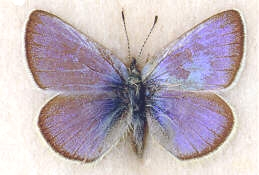
\includegraphics[scale=0.7]{images/xerces_blue.jpg}
                    \end{center}
                    \caption{Der Xerces Blue Schmetterling}
                    \label{fig:xerces_blue}
                \end{figure*}\par





        				\section{XML-Datenbanken}%Stefan
					Laut Pflichtenheft sollte die Datenspeicherung in einer XML-Datenbank erfolgen, da es sich bei den Daten grunds�tzlich nur um XML-Daten handelt. Eine weitere Einschr�nkung war die Voraussetzung, da� es sich um eine Open-Source-L�sung handelt. Die folgenden beiden Vertreter von XML-Datenbanken wurden zum Vergleich ausgew�hlt. Beide Alternativen stellen eine Implementierung der XML:DB-API \index{XML:DB-API} \cite{xmldb_api} bereit. Eine �bersichtliche Aufstellung aller weiteren verbreiteten XML-Datenbanken wurde von Ronald Bourret angefertigt \cite{xml_database_comparison}. 
					\subsection{Xindice}
						Xindice\index{Xindice} (gesprochen [zeen-dee-chay]) wird von der Apache Software Foundation\index{Apache Software Foundation} entwickelt und stellt eine Weiterentwicklung von \textit{dbXML 	1.0}\index{dbXML} dar. Die Anbindung an verschiedene Programmiersprachen ist durch ein XML-RPC Plugin\index{XML-RPC Plugin} gew�hrleitest. Speziell f�r Java ist eine XML:DB API Implementierung entwickelt worden. Zur Zeit werden XPATH\index{XPATH} als Anfragesprache und XML:DB-XUpdate\index{XML:DB-XUpdate} als �nderungssprache verwendet.\\
						Folgende Eigenschaften zeichnet Xindice aus :\\
						 \begin{itemize}
						 	\item{Strukturierung durch Collections : Dokumente werden in Collections gespeichert(entsprechen Verzeichnissen in einem Betriebssystem)}
						 	\item{XPATH Such-Engine : Zur Suche wird XPATH verwendet, das vom W3C(\url{http://www.w3.org/})\index{W3C} spezifiziert wurde. XPATH ist ein bew�hrter Anfrage-Standard auf XML-Dokumenten.}
						 	\item{Indezierung :  Zur Verbesserung der Suchperformance k�nnen Dokumentelemente etc. indexiert werden.}
						 	\item{XML:DB XUpdate Implementierung : M�glichkeit der serverseitgen Daten�nderung.}
						 	\item{XML:DB API Implementierung : Zur Verbundenheit von Java und XML wurde eine Java-Schnittstelle implementiert.}
						 	\item{Kommandozeilen-Befehle : Nahezu alle Funktionen der XML:DB API k�nnen auch durch Eingabe von Kommandos erfolgen.}
						 	\item{Modulare Architektur : Modularer Aufbau von Xindice zur einfachen Erweiterung und Integration in bestehenden Systeme.}
						 \end{itemize}
						F�r n�here Informationene siehe :\cite{xindice},\cite{xindice_admin_guide},\cite{xindice_user_guide},\cite{xindice_developer_guide},\cite{xindice_tools}.
					\subsection{eXist}
						eXist ist eine Open-Source\index{Open-Source} native XML-Datenbank (zur Zeit Version 1.0), die von Wolfgang M. Meyer entwickelt
						wurde. Wie bei der vorgestellten Alternative Xindice ist auch hier die M�glichkeit der Einbettung in anderer Applikationen, in
						eine Servlet-Engine sowie ein Stand-alone-Betrieb vorgesehen. F�r die Einbettung in einen Servlet-Container wird
						Jetty(\url{jetty.mortbay.org}) verwendet, wobei andere Servlet-Container ebenfalls eingesetzt werden k�nnen. eXist zeichnet sich
						durch folgende Eigenschaften aus:\\
						\begin{itemize}
							\item{Automatische Index-Erstellung : Index-Erstellung, um Performance zu steigern}
							\item{XPath/XQuery Such-Engine : Neben XPATH sind auch XQuery-Anfragen m�glich}
							\item{Volltextsuche : Mittels Indexierung performant gel�st}
							\item{XML:DB XUpdate : M�glichkeit um Daten serverseitig zu �ndern}
							\item{Zugriff �ber XML:DB API, HTTP, XML-RPC, SOAP, WebDAV : Verschiedenste Netzwerkanbindungen}
							\item{Backup/Restore Funktion : Backup der kompletten Datenbank mit allen Zugriffsbeschr�nkungen etc.}
							\item{Authorisierungsmechanismus : Ein an UNIX-Authorisierung angelehntes Verfahren(Jedoch nicht im XML:DB API Standard enthalten)}
						\end{itemize}
						F�r n�here Informationene siehe: \cite{xindice},\cite{exist_doc},\cite{exist_doc2},\cite{xml_data_management},\cite{xml_database_comparison}.						
					\subsection{Fazit}
						Der recht kurze �berblick der beiden vorgestellten XML-Datenbanken zeigt grunds�tzliche �bereinstimmungen sowie spezielle
						Unterscheidungen. Beide L�sungen sind native XML-Datenbanken, k�nnen leicht integriert werden und sind �ber die XML:DB API
						seitens Java ansteuerbar. eXist ist zus�tzlich in der Lage, automatisch einen Index zu erstellen und darauf Volltextsuchen
						durchzuf�hren. Weiterhin ist ein Benutzermanagement sowie eine Backup/Restore Funktionalit�t gegeben, die f�r das angehende
						Projekt unerl��lich sind. Insgesamt scheint eXist mehrere Features zu haben, die eventuell im Verlaufe des Projektes noch genutzt
						werden k�nnen. Ein Performance-Gegen�berstellung spricht ebenfalls f�r eXist. Diese Gegen�berstellung ist unter \cite{exist_doc2} zu finden.\\ 
						Insgesamt fiel die Entscheidung also auf die Open-Source L�sung 'eXist', die nun f�r die Datenhaltung sorgen wird.

                  \section{Konfigurationsmanagement}%Stefan
            \subsection{Buildmanagement}
                        \subsubsection{Allgemeines}
                            \paragraph{Was bedeutet Buildmanagement?}
                                Unter dem Stichwort \textit{Buildmanagement} ist der Prozess zwischen Entwicklung und Einsatz eines Softwareproduktes zu verstehen. Unter Einsatz eines Produktes ist hierbei nicht ausschlie�lich der Kundeneinsatz gemeint, vielmehr unterst�tzt dieser Prozess den stetigen Einsatz w�hrend der Entwicklung, z.B. zu Testzwecken.
                                Bestandteile dieses Prozesses sind u.a.
                                \begin{itemize}
                                    \item{Generierung von Kompilaten}
                                    \item{Strukturierung und Gew�hrleistung der Einsatzf�higkeit (Deployment)}
                                \end{itemize}           
                                In kleinen recht �berschaubaren Projekten wird diese Aufgabe sozusagen von den zur Entwicklung bereitgestellten Tools schon mit�bernommen. In umfangreicheren Projekten ist es jedoch notwendig, zur Erhaltung einer bestimmten Struktur und der    Handhabbarkeit, Werkzeuge einzusetzen, die es erm�glichen sehr detailiert und umfangreich das Erstellen eines Softwareproduktes zu �bernehmen. Im folgenden werden zwei Varianten von Build-Management Werkzeugen vorgestellt. Das erste, recht verbreitete und �ltere Werkzeug kommt aus der UNIX-Welt mit Namen \textit{make}. \\
                        \subsubsection{make}
                            \textbf{make : maintain, update, and regenerate related programs and files}\cite{make_doc}\\
                            Das \index{make}make Utility ist in der Hinsicht programmiersprachenunabh�ngig, solange ein Kompiler f�r die Konsole zur Verf�gung steht. Die weiteste
			    Verbreitung wurde durch die Programmiersprache 'C' und 'C++' geleistet. Make ist eine Konsolenanwendung , die als Argument ein \textit{makefile}
			    erh�lt, das die genauen Instruktionen beinhaltet. Ein \index{makefile} makefile dient h�ufig der Angabe, wie bestimmte Sourcen kompiliert und gelinkt
			    werden sollen. Da make als Buildmanagement Werkzeug nur der Vollst�ndigkeit halber aufgef�hrt wird, wird nun direkt zu einem abschlie�enden Beispiel �bergegangen.
                            \begin{figure*}[!htb]
                                \begin{center}
                                    \begin{Verbatim}[tabsize=2,frame=leftline,label=build.xml,numbers=left]
edit : main.o kbd.o command.o display.o \
   insert.o search.o files.o utils.o
    cc -o edit main.o kbd.o command.o display.o \
               insert.o search.o files.o utils.o
main.o : main.c defs.h
    cc -c main.c
kbd.o : kbd.c defs.h command.h
    cc -c kbd.c
command.o : command.c defs.h command.h
    cc -c command.c
display.o : display.c defs.h buffer.h
    cc -c display.c
insert.o : insert.c defs.h buffer.h
    cc -c insert.c
search.o : search.c defs.h buffer.h
    cc -c search.c
files.o : files.c defs.h buffer.h command.h
    cc -c files.c
utils.o : utils.c defs.h
    cc -c utils.c
clean :
    rm edit main.o kbd.o command.o display.o \
       insert.o search.o files.o utils.o            
                                    \end{Verbatim}                  
                        \end{center}
                            \caption{Einfaches make-file}
                        \label{makefile}
                            \end{figure*}\par                   
                            Diese Datei besteht aus mehreren Regeln, die nach folgender Struktur aufgebaut sind:\\
                            \textit{targets : prerequisites ; command command ...}\\
                            Das Beispiel \ref{makefile} soll verdeutlichen, da� das Erstellen einer ausf�hrbaren Datei namens 'edit' von 8 Objekt-Dateien abh�ngt, die wiederum von 8 C-Dateien und 3 Header-Dateien abh�ngen.
    
                        \subsubsection{ant}
                            \paragraph{Vorgehensweise/Systemvoraussetzungen}
                                Voraussetzungen f�r den Einsatz von Ant ist eine Java-Installation. N�heres unter \url{http://ant.apache.org/}. Wichtig im Anschluss ist das
				Setzen der Umgebungsvariablen \\
				\textit{ANT\_HOME=[Pfad zur Ant-Installation]} und Erweiterung der Variablen \textit{PATH}, um die ausf�hrbaren Ant-Dateien verf�gbar zu
				machen. Das Starten geschieht dann mittels des Aufrufes der ausf�hrbaren Datei \textit{ant}. Falls ant nicht im Verzeichnis, welches die build.xml
				enth�lt aufgerufen wird, so muss als Argument der Pfad zur build.xml angef�gt werden. Ansonsten reicht der alleinige Aufruf von 'ant'.
                    
                            \paragraph{Einf�hrung}  
                                Ein wesentlich j�ngeres Buildmanagement Werkzeug als 'make' kommt aus der Java-Welt und wird von der Apache-Group\cite{ant_doc} entwickelt und gepflegt. \index{ant} Ant ist ein java-basiertes Build-tool �hnlich dem Vorgestellten 'make'. Ant beseitigt die Abh�ngigkeit von der Konsole, ist XML-basiert und kann plattformunabh�ngig eingesetzt werden. Gerade bei der Entwicklung von Java-Applikationen ist Ant zu empfehlen, da es in erster Linie f�r diesen Einsatz entwickelt wurde. Da es auf XML basiert, ist es leicht, Ant-Skripte programmleserlich zu machen. XML als plattformunabh�ngiges Datenaustausch-/Beschreibungsformat ist zudem von denselben Grunds�tzen wie Java gepr�gt. Es handelt sich also um offensichtlich gut zusammenpassendes Duo, das im praktischen Einsatz seid Jahren bew�hrt ist.\\
                                Da Ant in dem angehenden Projekt verwendet wird, soll hier nun eine etwas ausf�hrlichere Einf�hrung gegeben werden, als es bei make geschah. Als Beispiel, das anschliessend beschrieben werden soll, dient das build-Skript des Projektes. Es ist im Anhang \ref{ant_code} zu finden

                            Angefangen mit der Deklaration, da� es sich um eine XML-Datei handelt, wird der Parser angeleitet, das Dokument zu verarbeiten. Die Root-Node \textit{Project} definiert das Arbeitsverzeichnis '.' und das default-target, welches aufgerufen wird, falls kein anderes target spezifiziert wird. Targets definieren also T�tigkeiten, die zumindest anf�nglich vom Benutzer vorgegeben werden. Im Folgenden werden die wichtigsten targets beschrieben :\\
                        \begin{itemize}
                            \item{usage: Das default-target, welches Auskunft �ber Namen und Beschreibung der 
                            anderen targets gibt}
                            \item{init: Im wesentlichen Variableninitialisierung, die von anfolgenden targets 
                            benutzt werden k�nnen}
                            \item{prepare: Dient der strukurellen Initialisierung, d.h. im wesentlichen 
                            Verzeichnisse anlegen etc.}
                            \item{do\_p30: Target, das alle wesentlichen T�tigkeiten ausf�hrt. Es leitet den Kompiliervorgang und das anschlie�ende Deployment ein.}
                            \item{start\_tooliban:  Startet die Clientanwendung, mittels der die implementierte Funktionalit�t bereitgestellt wird.}
                            \item{p30\_projektbericht: Zust�ndig f�r die Erstellung dieses Projektberichts}
                            \item{alle anderen: Spezielle targets, die bestimmte Aufgaben erledigen sollen}
                            \begin{itemize}
                                \item{p30\_compile: Kompilieren des src-Verzeichnisse}
                                \item{p30\_deploy: Erstellen eines Jar-Files mit Kopieroptionen}
                                \item{p30\_javadoc: Erstellung der Java-Dokumentation der Sourcen}
                                \item{start\_exist: Startet die eXist-Datenbank}
                                \item{stop\_exist: Stoppt die eXist-Datenbank}
                                \item{extract\_exist: Wird verwendet, um nach dem erstmaligen Checkout eine initiale Verzeichnisstruktur zu erstellen.}
                            \end{itemize}
                        \end{itemize}
                        Jedes target besitzt besondere Optionen, wobei folgende generell g�ltig sind:
                        \begin{itemize}
                            \item{depends : Gibt Abh�ngigkeiten zu anderen targets an, die dann automatisch 
                            aufgel�st werden}
                            \item{description : Beschreibung des anstehenden targets}
                        \end{itemize}
    
                \paragraph{Projektbezogenes Vorgehen}
                	Eine detailierte Beschreibung, wie das Buildmanagement im Projekt eingesetzt wird erfolgt im Anhang \ref{build_p30}.
        \subsection{Versionsmanagement}
                \subsubsection{CVS}
                    \paragraph{Was ist CVS?}
                        CVS\cite{cvs_doc} \index{cvs} steht f�r "`Concurrent Version Control"'. Es handelt sich hierbei also um ein System zur \textit{Versionskontrolle}
			beliebiger Daten. Angefangen mit einer initialen Version eines Datums werden im Laufe der Zeit �nderungen an diesem Datum vorgenommen, die zu einer neuen Version f�hren. Diese �nderungen werden mittels CVS verwaltet, so da� zu beliebiger Zeit jede Version anhand einer bestimmten Kennung wiederherstellbar ist. Der Begriff Version hat im Kontext CVS eine besondere Bedeutung, auf die sp�ter detailierter eingegangen wird (siehe \ref{cvs_version}). Der gerade beschriebene Ablauf l�sst sich nun auf eine Vielzahl von Dateien anwenden, die z.B. im Laufe eines Projektes von Bedeutung sind.\\
			Das CVS-System wird in eine Server- und eine Clientschicht unterteilt. Auf der Serverseite liegen in einem sogenannten \textit{Repository} \index{Repository} u.a. alle Informationen �ber die zeitliche �nderung einer Datei. Da die Arbeit auf den Daten des Repositories immer nur auf einer Kopie stattfindet, wird der Zugriff auf das Repository �ber einen Client erm�glicht. Der Client dient dem Zugriff und der Abgabe gewisser Kommandos bzgl. einer Datei.\\
                        Eine wichtige Eigenschaft stellt weiterhin die Konkurrenz dar. Sie verdeutlicht die M�glichkeit des konkurrierenden Arbeitens auf den Daten des
			Repositories. Es ist also ein Mehrbenutzerbetrieb vorgesehen. M�gliche Konflikte, die bei der Bearbeitung einer Datei von mehreren Personen zur gleichen
			Zeit auftreten k�nnen, werden prinzipiell als unwahrscheinlich angesehen. Diese Annahme bezeichnet den Vorgang des \textit{optimistischen Sperrens}\index{Optimistisches Sperren}. Es wird also davon ausgegangen, das immer nur eine Person eine Datei gleichzeitig bearbeitet. Falls dennoch ein
			Konflikt auftritt, wird serverseitig versucht, den Konflikt zu l�sen (\textit{merge}). Diese serverseitige Konfliktl�sung funktioniert solange bis mehrere
			�nderungen in derselben Zeile vorgenommen wurden. Einzig in diesem Fall wird die Konfliktl�sung an den jeweiligen Client weitergegeben, der dann manuell
			entscheiden muss, wie weiter vorgegangen werden soll.
                    \paragraph{Allgemeiner Umgang}
                        Es soll nun ein Umgang mit CVS beschrieben werden, z.B. im Einsatz eines Projektes. Die Beschreibung beschr�nkt sich jedoch auf die Benutzersicht. Jegliche administrativen Vorg�nge, wie Einrichtung, Benutzermanagement, etc. werden au�er Acht gelassen.\\
                        Vorab sollen folgende wichtige Funktionen erkl�rt werden, bevor ein Beispielszenario vorgestellt wird:
                            \subparagraph{cvs login}
                                Um den Zugang zu einem bestimmten Repository zu erlangen, wird eine Authentifizierung vorangestellt, in der das Repository mit Benutzernamen und
				Passwort verlangt werden.\\
                                Folgender Aufruf ist hierbei �blich :\\
                                \begin{Verbatim}[tabsize=2,frame=leftline,label=build.xml]
cvs -d:pserver:[username]@[servername]:[repository_path] login
                                \end{Verbatim}
                            \subparagraph{cvs checkout}
                                Nach einem erfolgreichen erstmaligen Einloggen wird eine Kopie des zu bearbeitenden Repositories angefordert.\\
                                Folgender Aufruf ist hierbei �blich :\\
                                \begin{Verbatim}[tabsize=2,frame=leftline,label=build.xml]
cvs -d:pserver:[username]@[servername]:[repository_path] checkout [module_name]
                                \end{Verbatim}
                            \subparagraph{cvs update}
                                Um �nderungen anderer Personen lokal auf eine bestehende Kopie zu erhalten wird ein Update-Proze� gestartet. Dieser Proze� kann rekursiv an jeder Stelle des Projekt-Verzeichnisbaumes durchgef�hrt werden. Es muss also nicht immer das komplette Projekt untersucht werden. Dateiangaben sind ebenso m�glich wie Verzeichnisangaben. Ein Update-Proze� beinhaltet auch immer ein Abgleich der eigenen �nderungen mit denen anderer.\\
                                Folgender Aufruf ist hierbei �blich :\\
                                \begin{Verbatim}[tabsize=2,frame=leftline,label=build.xml]
cvs -d:pserver:[username]@[servername]:[repository_path] update [local_path]
                                \end{Verbatim}
                            \subparagraph{cvs add}
                                Im Laufe eines Projektes ist es n�tig neben �nderungen auch neue initiale Dateien einzustellen.\\
                                Folgender Aufruf ist hierbei �blich :\\
                                \begin{Verbatim}[tabsize=2,frame=leftline,label=build.xml]
cvs -d:pserver:[username]@[servername]:[repository_path] add [file_path]
                                \end{Verbatim}
                            \subparagraph{cvs remove}
                                Ebenso das L�schen von nicht mehr ben�tiger Dateien ist sinnvoll, da z.B. keine Umbenennung-Funktionen von Dateien bereitgestellt wird. Wichtig hierbei ist, da� Dateien serverseitig nur als gel�scht markiert werden, so da� der explizite Zugriff m�glich bleibt. Weiterhin ist es nicht m�glich, Verzeichnisse zu l�schen bzw. als gel�scht zu markieren.\\
                                Folgender Aufruf ist hierbei �blich :\\
                                \begin{Verbatim}[tabsize=2,frame=leftline,label=build.xml]
cvs -d:pserver:[username]@[servername]:[repository_path] remove [file_path]
                                \end{Verbatim}
                            \subparagraph{cvs commit}
                                Jede bisherige �nderungsoperation wird erst global gepr�ft(siehe cvs update) nachdem eine Best�tigung erfolgt. Diese Best�tigung wird wiederum rekursiv an beliebiger Stelle im Projektpfad gestellt. Dieser Schritt ist also der Entscheidende bei einer �nderung .\\
                                Folgender Aufruf ist hierbei �blich :\\
                                \begin{Verbatim}[tabsize=2,frame=leftline,label=build.xml]
cvs -d:pserver:[username]@[servername]:[repository_path] commit
                                \end{Verbatim}
	
			\paragraph{Version - Revision - Variante - Release}
		    \label{cvs_version}
		    \subparagraph{Version}
		    	Unter einer Version wird im CVS-Kontext eine Auspr�gung eines Datums verstanden, das sich von anderen unterscheidet. Abweichungen zwischen Versionen entstehen z.B.
			durch funktionale Erweiterung, Fehlerbehebung u.a..
		    \subparagraph{Revision vs. Variante}
		    	Eine Revision stellt das Ergebnis einer �berarbeitung einer Version dar. Es handelt sich hierbei also um eine evolution�re Entwicklung. Eine Variante dagegen teilt die evolution�re eindeutige Entwicklung in mehrere Richtungen (z.B. Parallelentwicklungen Betriebssystemabh�ngig). Bei verschiedenen Varianten sind nicht-funktionale Abweichungen festzustellen, wobei eine funktionale Identit�t gew�hrleistet werden sollte. Folgendes Bild (\ref{fig:cvs_variante_revision}) veranschaulicht den Zusammenhang
			nochmals, wobei auch die Revisionsnummern angegeben sind - zum Vergleich.
                        \begin{figure*}[!htb]
                            \begin{center}
                                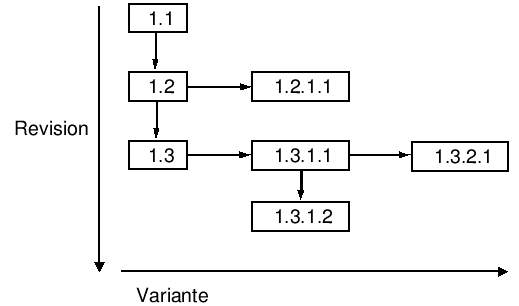
\includegraphics[scale=0.7]{images/cvs_revisionen.png}
                            \end{center}
                            \caption{Variante/Revision}
                            \label{fig:cvs_variante_revision}
                        \end{figure*}\par
		    \subparagraph{Release}
		    	Im Falle eines Softwareproduktes, welches durch CVS gehalten wird, wird jede Ausbringung des Produktes an den Kunden als Release bezeichnet. Ein Release kann somit eine einsatzbereite funktionale Erweiterung eines Softwareproduktes darstellen. Allgemein ist hierbei der Kundenbezug pr�gend.
			\paragraph{Projektbezogenes Vorgehen}
				Eine detaillierte Beschreibung, wie konkret CVS im Projekt genutzt wird, findet sich im Anhang \ref{cvs_p30}. 



%%%%%%%%%%%%%%%%%%%%%%%%%%%%%%%%%%%%%%%%%%%%%%%%%%%%%%%%%%%%%%%
% Anforderungsanalyse
%%%%%%%%%%%%%%%%%%%%%%%%%%%%%%%%%%%%%%%%%%%%%%%%%%%%%%%%%%%%%%% 

    \chapter{Anforderungsanalyse}
    
\section{Vorgehensmodell}%Thorsten
        Das Entwicklungsteam hat sich bei der Wahl des Vorgehensmodells \index{Vorgehensmodell} f\"ur das Modell der 
    evolution\"aren Softwareentwicklung \index{Softwareentwicklung, evolution\"are} entschieden. 
    Bei der evolution\"aren Softwareentwicklung wird anhand der Vorgaben
        des Auftraggebers ein Prototyp \index{Prototyp} entwickelt. Dieser Prototyp wird nach Fertigstellung dem Auftraggeber 
        vorgestellt, wobei dieser nun die M\"oglichkeit hat zu bewerten, ob der Prototyp seinen W\"unschen
        und Vorstellungen entspricht. Anhand seiner Kritik wird der Prototyp verbessert und erneut dem Kunden
        zur Ansicht gereicht; solange bis dieser mit dem Ergebnis zufrieden ist.

        Die Entscheidung, dem Vorgehensmodell der evolution\"aren Softwareentwicklung den Vorzug zu geben,
        wurde aus folgenden Gr\"unden getroffen:

        \begin{itemize}
          \item Das Team ist noch relativ unerfahren auf dem Gebiet der Softwareentwicklung
          \item Die einzelnen Entwickler haben in dieser Form noch nicht zusammen gearbeitet
          \item Keiner der Beteiligten hatte zu Beginn des Projektes Erfahrungen innerhalb des 
            Anwendungsgebietes
        \end{itemize}

        Daher bot sich die evolution\"are Entwicklung an, weil man dabei recht schnell zu sichtbaren Ergebnissen 
        gelangt. Dadurch kann im Team Sicherheit gewonnen werden. Zum einen, da man Erkenntnisse dar\"uber
        erh\"alt, ob die angedachten Ideen und Vorstellungen praktisch durchgef\"uhrt werden k\"onnen bzw.
        konnten. Zum anderen, da man engen Kontakt mit dem Auftraggeber pflegen kann und Best\"atigung 
        bekommt, ob die bisherige Leistung den Forderungen entspricht.


        \section{Anwendungsf�lle}%Thorsten
      An dieser Stelle werden die m\"oglichen Anwendungsf\"alle (engl. Use Cases)\index{Anwendungsfall} der Benutzer 
      grafisch als auch textuell dargestellt.
      Ein Anwendungsfall beschreibt eine Menge von Aktivit\"aten eines Systems aus Sicht seiner Akteure, die f\"ur die
      Akteure \index{Akteur}zu einem wahrnehmbaren Ergebnis f\"uhren.\cite{oestereich}

      Genau betrachtet gibt es nur zwei Benutzergruppen; der Benutzer \index{Benutzer}mit administrativen Rechten 
      und der Benutzer ohne
      solche Rechte. Im Folgenden werden diese beiden Benutzerarten einfach nur als ``Administrator'' \index{Administrator}
      und ``Benutzer'' bezeichnet.

      \begin{figure*}[!htb]
                        \begin{center}
                            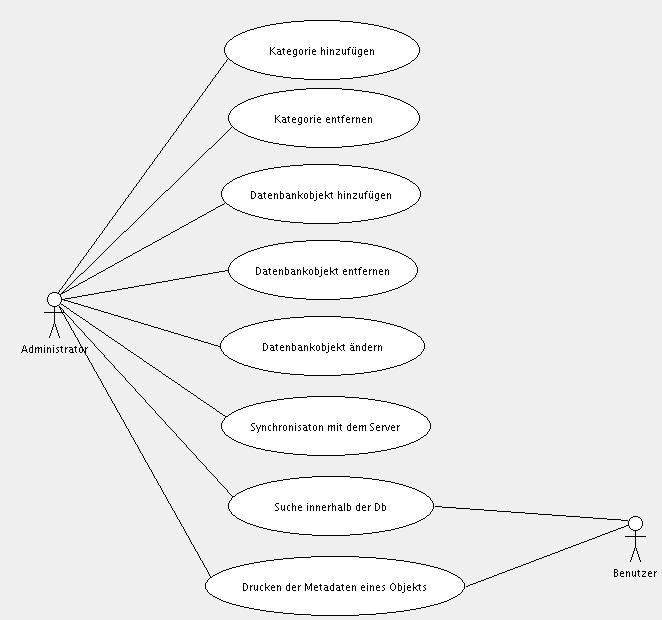
\includegraphics[scale=0.6]{images/Usecase.jpg}
                        \end{center}
                        \caption{Anwendungsf\"alle}
                        \label{fig:Usecase}
                    \end{figure*}\par


      Abbildung \ref{fig:Usecase} zeigt die Anwendungsf\"alle f\"ur die beiden Benutzergruppen. Es folgt eine textuelle
      Kurzbeschreibung der einzelnen F\"alle:

      \begin{enumerate}
        \item Kategorie \index{Kategorie}hinzuf\"ugen
            \begin{itemize} 
          \item Akteur: Administrator
          \item Vorbedingung: gew\"unschte Kategorie ist nicht in Kategorienliste enthalten
          \item Nachbedingung: Kategorienliste wird um die neue Kategorie erweitert
          \item Ablauf: Der Akteur gibt in einem Dialog den Name der neuen Kategorie an
            \end{itemize}
         
         \item Kategorie entfernen
            \begin{itemize}
                  \item Akteur: Administrator
                  \item Vorbedingung: der zu entfernenden Kategorie ist kein Objekt \index{Objekt} zugeordnet
                  \item Nachbedingung: Kategorie wird aus der Kategorienliste entfernt
                  \item Ablauf: Der Akteur w\"ahlt aus der ihm angezeigten Liste die betreffende Kategorie
          \item Fehlersituation: die zu entfernende Kategorie ist nicht leer, ein Entfernen ist nicht m\"oglich
                \end{itemize}

         \item Datenbankobjekt hinzuf\"ugen
             \begin{itemize}
                  \item Akteur: Administrator
                  \item Vorbedingung: keine
                  \item Nachbedingung: Objekt wird in die Datenbank aufgenommen
                  \item Ablauf: Der Aktuer w\"ahlt die entsprechende Objektart und die gew\"unschte Kategorie aus. 
            Er gibt anschlie{\ss}end die ben\"otigten Metadaten des Objekts ein.
                \end{itemize}

          \item Datenbankobjekt entfernen
          \begin{itemize}
                  \item Akteur: Administrator
                  \item Vorbedingung: zu entfernendes Objekt existiert in der Datenbank
                  \item Nachbedingung: Objekt wird aus Datenbank entfernt
                  \item Ablauf: Der Akteur sucht das entsprechende Objekt in der Datenbank und kann es dann
            entfernen
                \end{itemize}

          \item Datenbankobjekt \"andern
                  \begin{itemize}
                  \item Akteur: Administrator
                  \item Vorbedingung: zu \"anderdes Objekt existiert in der Datenbank
                  \item Nachbedingung: Metadaten \index{Metadaten} des entsprechenden Objekts werden ge\"andert
                  \item Ablauf: Der Akteur sucht das entsprechende Objekt in der Datenbank und kann dann die
            gew\"unschten \"Anderungen der Metadaten vornehmen.
                \end{itemize}

          \item Synchronisation \index{Synchronisation}mit dem Server
                  \begin{itemize}
                  \item Akteur: Administrator
                  \item Vorbedingung: keine
                  \item Nachbedingung: die neuen Eintr\"age werden dem Server \"ubermittelt und im Gegenzug neue 
            Servereintr\"age dem Client
                  \item Ablauf: Der Akteur w\"ahlt aus der ihm vorliegenden Serverliste den entsprechenden Server und kann
            sich dann mit ihm synchronisieren.
          \item Fehlersituation: Der Akteur hat keine administrativen Rechte auf dem gew\"ahlten Server.
                \end{itemize}

          \item Suchen innerhalb der Datenbank
                  \begin{itemize}
                  \item Akteure: Administrator, Benutzer
                  \item Vorbedingung: keine
                  \item Nachbedingung: keine
                  \item Ablauf: Der Akteur kann anhand eines Suchbegriffs aus den Metadaten Objekte suchen
          \item Fehlersituation: Der Suchbegriff konnte nicht in der Datenbank gefunden werden.
                \end{itemize}

          \item Drucken der Metadaten eines Objekt
                  \begin{itemize}
                  \item Akteure: Administrator, Benutzer
                  \item Vorbedingung: zu druckendes Objekt wurde ausgew\"ahlt
                  \item Nachbedingung: keine
                  \item Ablauf: Der Akteur kann das zur Zeit ausgew\"ahlte Objekt ausdrucken lassen
                \end{itemize}

      \end{enumerate}







        \section{Pflichtenheft}%Thorsten    
    Das hier dargestellte Pflichtenheft \index{Pflichtenheft}orientiert sich an den Vorgaben des 
    Buches ``Lehrbuch f\"ur Software-Technik'' von Helmut Balzert \cite{balzert}.

    \subsection{Zielbestimmungen}
       Unser Auftraggeber soll durch das Produkt in der Lage sein, seinen Literaturbestand effizient zu verwalten.
       
       \subsubsection{Mu{\ss}kriterien}
          \begin{itemize}
        \item Hinzuf\"ugen und Entfernen von Objekten \index{Objekt} zum Bestand
        \item Als Objekte gelten \index{Buch}B\"ucher, \index{Zeitschrift}Zeitschriften, Artikel, Audio- und Filmdateien
        \item Kategorisierung \index{Kategorie} des Bestands
        \item Suchfunktion anhand von Metadaten \index{Metadaten}
        \item Druckfunktion auf einem Postscript-Drucker \index{Drucker} \index{Postscript}
        \item Web-Client zum Durchsuchen der Datenbank mittels WWW \index{World Wide Web (WWW)}
      \end{itemize}
    \subsubsection{Wunschkriterien}
       \begin{itemize}
         \item Volltextsuche
         \item Import von anderen Datenformaten
         \item Export im BibTeX-Format \index{BibTeX}
         \item Hinzunahme weitere Objektarten bei Bedarf
       \end{itemize}

    \subsubsection{Abgrenzungskriterien}
       Obwohl f\"ur betriebsfremde Personen eine Ausleihm\"oglichkeit besteht, wird eine Ausleihverwaltung
       nicht realisiert.

    \subsection{Produkteinsatz}
       Das Produkt dient zur Verwaltung des gesamten Literaturbestands. Einzelne Mitarbeiter k\"onnen ihren
       individuellen Bestand pflegen und in den Gesamtbestand einflie{\ss}en lassen. Dieser kann von jedem
       Angestellten durchsucht werden, um den Standort des gesuchten Objekts ausfindig zu machen. Weiterhin
       ist es betriebsfremden Personen gestattet, die Datenbank mittels eines Web-Clients \"uber das WWW
       zu durchsuchen.

    \subsection{Produktumgebung}
       Das Produkt unterliegt einer Client-Server Architektur.\index{Client-Server Architektur}

       \subsubsection{Software}
          \begin{itemize}
             \item Betriebssystem: jedes, auf dem eine ``Sun Microsystems Java Runtime Engine'' lauff\"ahig ist \index{Java}

         \item Sonstige Software: Sun Microsystems \index{Sun Microsystems}Java Runtime Engine 
           (mindestens Version 1.4), eXist XML Datenbank
      \end{itemize}
       
       \subsubsection{Hardware}
          Sowohl der Server als auch jeder Client ben\"otigt lediglich die Hardware, die n\"otig ist, obige
      Software-Kriterien zu erf\"ullen. F\"ur die Verbindung von Server und Clients wird ein TCP/IP-Netzwerk
      ben\"otigt. \index{TCP/IP}

    \subsection{Produktfunktionen}
       \begin{enumerate}
     \item Verwaltung von Benutzergruppen mit Passw\"ortern \index{Passwort}
     \item Passwortabfrage beim Start des Programms
     \item Hinzuf\"ugen und Enfernen von Kategorien \index{Kategorie}
     \item Hinzuf\"ugen eines Objekts \index{Objekt}
       \begin{enumerate}
         \item Bestimmung der Objektart durch den Benutzer
         \item Bestimmung der Kategorie des Objekts durch den Benutzer
         \item Eingabe der ben\"otigten Metadaten durch den Benutzer
         \item Erzeugung einer eineindeutigen Signatur f\"ur das Objekt mit Hilfe der Kategorie durch das System
         \item Speicherung des Objekts in der Datenbank
       \end{enumerate}
     \item Entfernen eines Objekts
     \item Suchen eines Objektes anhand von Metadaten \index{Metadaten}
     \item \"Andern der Metadaten eines Objekt
     \item \"Ubermittlung der Daten des  pers\"onlichen Bestands an den Server (``Synchronisation'')\index{Synchronisation}
     \item Auswahl verschiedener Datenbankserver f\"ur den individuellen Gebrauch
     \item Erstellen einer Individualliste aus allen Datenbanken, die dem Benutzer zur Verf\"ugung stehen 
       \index{Individualliste}
         \item Drucken der Metadaten eines Objekts
         \item Import anderer Datenformate (insb. Excel)
         \item Export im BibTeX-Format \index{BibTeX}


       \end{enumerate}

    \subsection{Produktdaten}
       Alle Objektdaten werden im XML-Format gespeichert und halten sich so weit wie m\"oglich an die Vorgaben des 
       \index{Dublin Core} Dublin Core (vergl. \ref{dublin}). 

      


    \subsection{Benutzungsoberf\"ache} 
       Bei der Gestaltung der Benutzungsoberfl\"ache wird dem Entwicklungsteam 
       grunds\"atzlich freie Hand gelassen. \index{Oberfl\"ache, grafisch}
       Gefordert ist lediglich eine men\"uorientierte graphische Benutzungsoberfl\"ache (GUI), die haupts\"achlich 
       mit der Maus zu bedienen ist, trotzdem auch ohne Maus bedienbar bleibt. Durch die evolution\"are 
       Softwareentwicklung \index{Softwareentwicklung, evolution\"are} kann der erstellte und immer wieder 
       aktualisierte Prototyp \index{Prototyp} dem Auftraggeber zur Ansicht
       vorgelegt werden und so die Oberf\"ache st\"andig nach seinen W\"unschen verbessert werden.

    \subsection{Entwicklungsumgebung}

       \subsubsection{Software} \label{software}
          \begin{itemize}
        \item Als Programmiersprache wird Java \index{Java}verwendet. Ben\"otigt wird das ``Java Development Kit'' der Firma
          Sun Microsystems\footnote{\url{http://java.sun.com}} (mindestens Version 1.4).\index{Sun Microsystems}
        \item Als Programmierumgebung wird ``Eclipse'' von der Eclipse Foundation \index{Eclipse}
          empfohlen\footnote{\url{http://www.eclipse.org}}. Die Benutzung ist jedoch nicht zwingend.
        \item Als XML-Datenbank wird die Open-Source Datenbank ``eXist'' \index{Open-Source} \index{eXist}
          eingesetzt\footnote{\url{http://exist.sourceforge.net}}.
        \item Das Projekt betreffende Dokumente werden mit \LaTeX\ erstellt. \index{\LaTeX}
        \item Zum Versionsmanagement und zur Zusammenarbeit der beteilligten Entwickler wird CVS (Concurrent Version
          System) benutzt\footnote{\url{http://www.cvshome.org}}. \index{cvs}
      \end{itemize}

    \subsubsection{Hardware}
       Grunds\"atzlich wird keine spezielle Hardware erforderlich. Einziger Anspruch an die Hardware ist, dass die
       unter \ref{software} aufgef\"uhrten Programme und Werkzeuge einsetzbar sind.





